

\subsection{Library \og decorations.pathmorphing \fg}

\label{lib-morph}
\begin{center}
\RRR{48-2}
\end{center}

\subsubsection{\og lineto \fg}

\begin{tabular}{|c|c|c|} \hline  
\begin{tikzpicture}
\draw [dotted,red](0,0) -- (2,2) ;
\draw [decorate,decoration=lineto]
(0,0) -- (2,2) ;
\end{tikzpicture}
&  
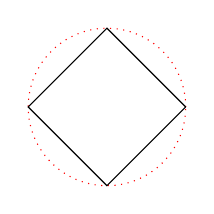
\begin{tikzpicture}
\draw [dotted,red] (1,1) circle (1);
\draw [decorate,decoration=lineto]
(1,1) circle (1); 
\end{tikzpicture}
&  
\begin{tikzpicture}
\draw [dotted,red]
(0,0)  arc (0:180:3 and 2) ;
\draw [decorate,decoration=lineto]
(0,0)  arc (0:180:3 and 2);
\end{tikzpicture}
\\ \hline  
(0,0) - - (2,2) & (1,1) circle (1) & (0,0)  arc (0:180:3 and 2)\\ \hline 
\end{tabular}

\subsubsection{ \og  straight zigzag \fg}

\begin{tabular}{|c|c|c|} \hline 
\multicolumn{3}{|c|}{\BSS{draw}[decorate,\RDD{decoration}=\RDDX{straight zigzag}{decoration}] (0,0) - - (2,2) ;}
\\ \hline 
\begin{tikzpicture}
\draw [dotted,red](0,0) -- (2,2) ;
\draw [decorate,decoration=straight zigzag](0,0) -- (2,2) ;
\end{tikzpicture}
&  
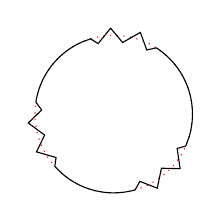
\begin{tikzpicture}
\draw [dotted,red] (1,1) circle (1);
\draw [decorate,decoration=straight zigzag](1,1) circle (1); 
\end{tikzpicture}
&  
\begin{tikzpicture}
\draw [dotted,red]
(0,0)  arc (0:180:3 and 2);
\draw [decorate,decoration=straight zigzag]
(0,0)  arc (0:180:3 and 2);
\end{tikzpicture}
\\ \hline  
(0,0) - - (2,2) & (1,1) circle (1) & (0,0)  arc (0:180:3 and 2); \\ 
\hline 
\end{tabular}

\bigskip

\begin{tabular}{|l|c|c|} \hline 
\multicolumn{2}{|c|}{\BSS{draw}[decorate,decoration=\AC{straight zigzag,\RDD{meta-segment length}=2cm}] (0,0) - - (10,0);}& \dft
 \\ \hline 
\RDD{meta-segment length}=2cm
&  
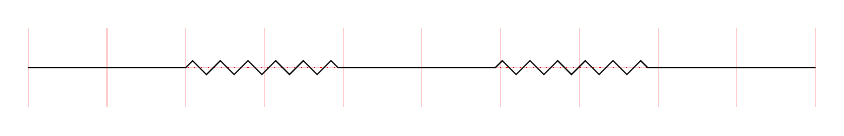
\begin{tikzpicture}[baseline=0pt]
\draw[red!20] (0,-0.5) grid (10,0.5);
\draw[dotted,red] (0,0) -- (10,0);
\draw[decorate,decoration={straight zigzag,meta-segment length=2cm}] (0,0) -- (10,0);
\end{tikzpicture}
& 1cm
\\ \hline  
\RDD{amplitude}=0.5cm
&  
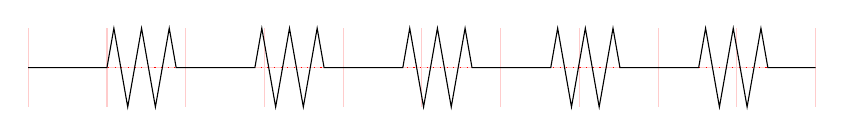
\begin{tikzpicture}[baseline=0pt]
\draw[red!20] (0,-0.5) grid (10,0.5);
\draw[dotted,red] (0,0) -- (10,0);
\draw[decorate,decoration={straight zigzag,amplitude=0.5cm}] (0,0) -- (10,0);
\end{tikzpicture}
& 2.5pt
\\ \hline 
\RDD{segment length}=1cm
& 
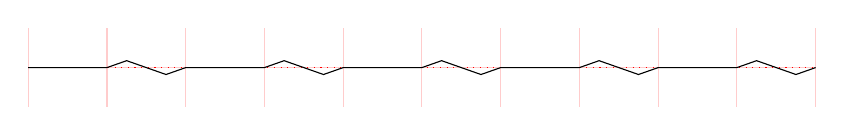
\begin{tikzpicture}[baseline=0pt]
\draw[red!20] (0,-0.5) grid (10,0.5);
\draw[dotted,red] (0,0) -- (10,0);
\draw[decorate,decoration={straight zigzag,segment length=1cm}] (0,0) -- (10,0);
\end{tikzpicture}
& 10pt
\\ \hline 
\end{tabular}

\bigskip

\begin{tabular}{|c|c|c|} \hline
\multicolumn{3}{|c|}{ \BSS{draw}[decorate,decoration=}\\
\multicolumn{3}{|c|}{\AC{straight zigzag,\RDD{meta-segment length}=0.5cm}] (1,1) circle (1); }
 \\ \hline 
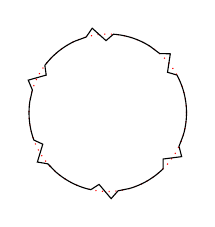
\begin{tikzpicture}[baseline=0pt]
\draw [dotted,red](1,1) circle (1); 
\draw [decorate,decoration={straight zigzag,meta-segment length=0.5cm}]
(1,1) circle (1); 
\end{tikzpicture}
&  
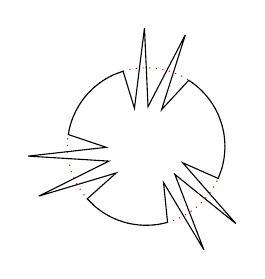
\begin{tikzpicture}[baseline=0pt]
\draw [dotted,red](1,1) circle (1); 
\draw [decorate,decoration={straight zigzag,amplitude=0.5cm}]
(1,1) circle (1); 
\end{tikzpicture}
&  
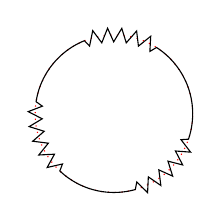
\begin{tikzpicture}[baseline=0pt]
\draw [dotted,red](1,1) circle (1); 
\draw [decorate,decoration={straight zigzag,segment length=5pt}]
(1,1) circle (1); 
\end{tikzpicture}
\\ \hline 
 \RDD{meta-segment length}=2cm & \RDD{amplitude}=0.5cm & \RDD{segment length}=5pt 
\\ \hline 
\end{tabular}

\subsubsection{\og random steps \fg }
\label{alea}

\begin{tabular}{|c|c|c|} \hline  
\multicolumn{3}{|c|}{\BSS{draw}[decorate,\RDD{decoration}=\RDDX{random steps}{decoration}] (0,0) - - (2,2) ;}
\\ \hline 
\begin{tikzpicture}
\draw [dotted,red](0,0) -- (2,2) ;
\draw [decorate,decoration=random steps]
(0,0) -- (2,2) ;
\end{tikzpicture}
&  
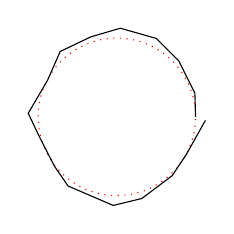
\begin{tikzpicture}
\draw [dotted,red] (1,1) circle (1);
\draw [decorate,decoration=random steps]
(1,1) circle (1); 
\end{tikzpicture}
&  
\begin{tikzpicture}
\draw [dotted,red]
(0,0)  arc (0:180:3 and 2);
\draw [decorate,decoration=random steps]
(0,0)  arc (0:180:3 and 2);
\end{tikzpicture}
\\ \hline  
(0,0) -- (2,2) & (1,1) circle (1) & (0,0)  arc (0:180:3 and 2)\\ 
\hline 
\end{tabular}

\bigskip

\begin{tabular}{|l|c|c|} \hline 
\multicolumn{2}{|c|}{\BSS{draw}[decorate,decoration=\AC{random steps,\RDD{segment length}=2cm}] (0,0) - - (10,0);} & \dft
\\ \hline 
\RDD{segment length}=2pt
&  
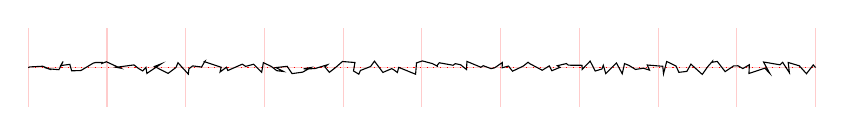
\begin{tikzpicture}[baseline=0pt]
\draw[red!20] (0,-.5) grid (10,.5);
\draw[dotted,red] (0,0) -- (10,0); \draw[decorate,decoration={random steps,segment length=2pt}] (0,0) -- (10,0);
\end{tikzpicture}
& 10pt \\
\RDD{segment length}=1cm
&  
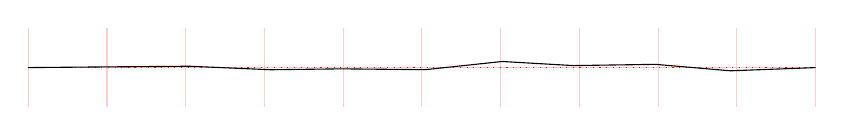
\begin{tikzpicture}[baseline=0pt]
\draw[red!20] (0,-.5) grid (10,.5);
\draw[dotted,red] (0,0) -- (10,0); \draw[decorate,decoration={random steps,segment length=1cm}] (0,0) -- (10,0);
\end{tikzpicture}
&
\\ \hline  
\RDD{amplitude}=0.5cm
&  
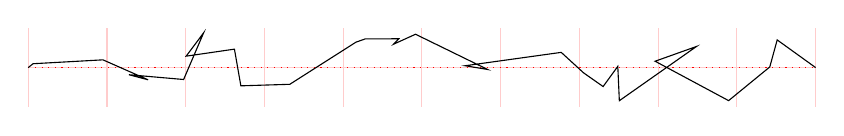
\begin{tikzpicture}[baseline=0pt]
\draw[red!20] (0,-.5) grid (10,.5);
\draw[dotted,red] (0,0) -- (10,0); \draw[decorate,decoration={random steps,amplitude=0.5cm}] (0,0) -- (10,0);
\end{tikzpicture}
& 2.5pt
\\ \hline 
\parbox{4cm}{
\RDD{amplitude}=0.5cm\\
,\RDD{segment length}=1cm}
&  
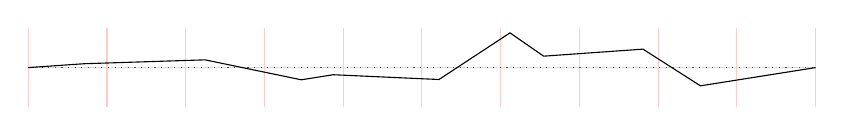
\begin{tikzpicture}[baseline=0pt]
\draw[red!20] (0,-.5) grid (10,.5);
\draw[dotted,red] (0,0) -- (10,0); \draw[decorate,decoration={random steps,amplitude=0.5cm,segment length=1cm}] (0,0) -- (10,0);
\end{tikzpicture}
&
\\ \hline 
\end{tabular} 

\bigskip

\begin{tabular}{|c|c|c|} \hline  
\multicolumn{3}{|c|}{ \BSS{draw}[decorate,decoration= 
\AC{random steps,\RDD{segment length}=2cm}] (1,1) circle (1); }
 \\ \hline 
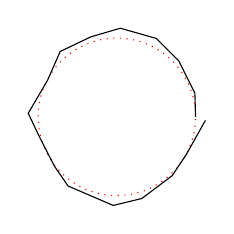
\begin{tikzpicture}
\draw [dotted,red](1,1) circle (1);
\draw [decorate,decoration={random steps,meta-segment length=2cm}]
(1,1) circle (1); 
\end{tikzpicture}
&  
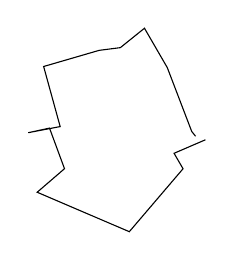
\begin{tikzpicture}
\draw [decorate,decoration={random steps,amplitude=0.5cm}]
(1,1) circle (1); 
\end{tikzpicture}
&  
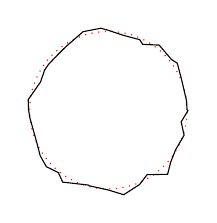
\begin{tikzpicture}
\draw [dotted,red](1,1) circle (1);
\draw [decorate,decoration={random steps,segment length=5pt}]
(1,1) circle (1); 
\end{tikzpicture}
\\ \hline 
 \RDD{meta-segment length}=2cm & \RDD{amplitude}=0.5cm & \RDD{segment length}=5pt 
\\ \hline 
\end{tabular} 

\subsubsection{\og saw \fg }

\begin{tabular}{|c|c|c|} \hline 
\multicolumn{3}{|c|}{\BSS{draw}[decorate,\RDD{decoration}=\RDDX{saw}{decoration}] (0,0) - - (2,2) ;}
 \\ \hline 
\begin{tikzpicture}
\draw [dotted,red](0,0) -- (2,2) ;
\draw [decorate,decoration=saw]
(0,0) -- (2,2) ;
\end{tikzpicture}
&  
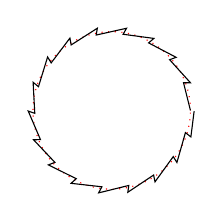
\begin{tikzpicture}
\draw [dotted,red] (1,1) circle (1);
\draw [decorate,decoration=saw]
(1,1) circle (1); 
\end{tikzpicture}
&  
\begin{tikzpicture}
\draw [dotted,red]
(0,0)  arc (0:180:3 and 2);
\draw [decorate,decoration=saw]
(0,0)  arc (0:180:3 and 2);
\end{tikzpicture}
\\ \hline  
(0,0) - - (2,2) & (1,1) circle (1) & (0,0)  arc (0:180:3 and 2);\\ 
\hline 
\end{tabular}

\bigskip

\begin{tabular}{|l|c|c|} \hline 
\multicolumn{2}{|c|}{\BSS{draw}[decorate,decoration=\AC{saw,\RDD{meta-segment length}=0.5cm}] (0,0) - - (10,0);} & \dft
 \\ \hline 
\RDD{segment length}=0.5cm
&  
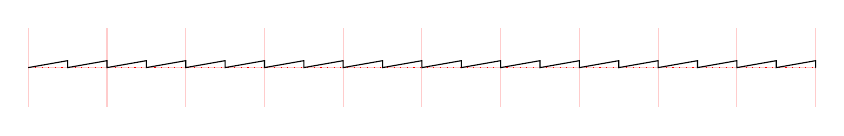
\begin{tikzpicture}[baseline=0pt]
\draw[red!20] (0,-0.5) grid (10,0.5);
\draw[dotted,red] (0,0) -- (10,0); \draw[decorate,decoration={saw,segment length=0.5cm}] (0,0) -- (10,0);
\end{tikzpicture}
& 10 pt \\ 
\RDD{segment length}=2cm
&  
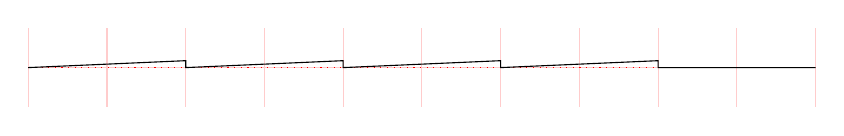
\begin{tikzpicture}[baseline=0pt]
\draw[red!20] (0,-0.5) grid (10,0.5);
\draw[dotted,red] (0,0) -- (10,0); \draw[decorate,decoration={saw,segment length=2cm}] (0,0) -- (10,0);
\end{tikzpicture}
&  \\ \hline 
\RDD{amplitude}=0.5cm
&  
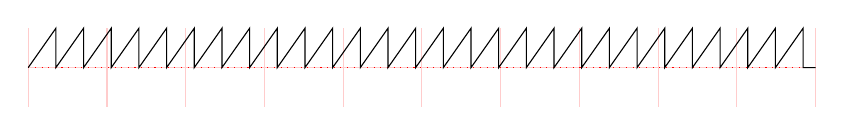
\begin{tikzpicture}[baseline=0pt]
\draw[red!20] (0,-0.5) grid (10,0.5);
\draw[dotted,red] (0,0) -- (10,0);\draw[decorate,decoration={saw,amplitude=0.5cm}] (0,0) -- (10,0);
\end{tikzpicture}
& 2.5 pt \\ \hline 
\end{tabular}

\bigskip

\begin{tabular}{|c|c|c|} \hline 
\multicolumn{3}{|c|}{ \BSS{draw}[decorate,decoration=\AC{saw,\RDD{segment length}=20pt}] (1,1) circle (1); }
 \\ \hline  
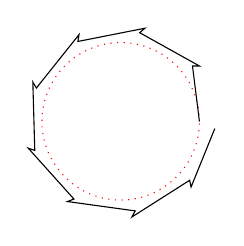
\begin{tikzpicture}
\draw [dotted,red](1,1) circle (1);
\draw [decorate,decoration={saw,segment length=20pt}]
(1,1) circle (1); 
\end{tikzpicture}
&  
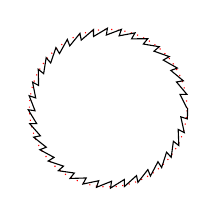
\begin{tikzpicture}
\draw [dotted,red](1,1) circle (1);
\draw [decorate,decoration={saw,segment length=5pt}]
(1,1) circle (1); 
\end{tikzpicture}
&  
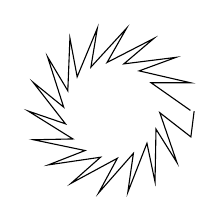
\begin{tikzpicture}
\draw [decorate,decoration={saw,amplitude=0.5cm}]
(1,1) circle (1); 
\end{tikzpicture}
\\ \hline 
\RDD{segment length}=20pt & \RDD{segment length}=5pt & \RDD{amplitude}=0.5cm 
\\ \hline 
\end{tabular}

\subsubsection{\og zigzag \fg }

\begin{tabular}{|c|c|c|} \hline  
\multicolumn{3}{|c|}{\BSS{draw}[decorate,\RDD{decoration}=\RDDX{zigzag}{decoration}] (0,0) - - (2,2) ;}
\\ \hline 
\begin{tikzpicture}
\draw [dotted,red](0,0) -- (2,2) ;
\draw [decorate,decoration=zigzag]
(0,0) -- (2,2) ;
\end{tikzpicture}
&  
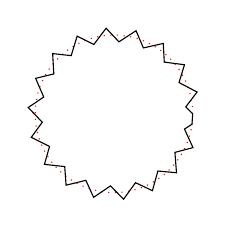
\begin{tikzpicture}
\draw [dotted,red] (1,1) circle (1);
\draw [decorate,decoration=zigzag]
(1,1) circle (1); 
\end{tikzpicture}
&  
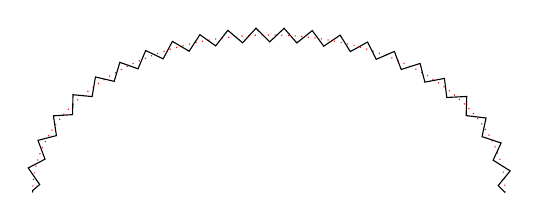
\begin{tikzpicture}
\draw [dotted,red]
(0,0)  arc (0:180:3 and 2);
\draw [decorate,decoration=zigzag]
(0,0)  arc (0:180:3 and 2);
\end{tikzpicture}
\\ \hline  
(0,0) - - (2,2) & (1,1) circle (1) & (0,0)  arc (0:180:3 and 2);\\ 
\hline 
\end{tabular}

\bigskip

\begin{tabular}{|l|c|c|} \hline 
\multicolumn{2}{|c|}{\BSS{draw}[decorate,decoration=\AC{zigzag,\RDD{meta-segment length}=2cm}] (0,0) - - (10,0);} & \dft
 \\ \hline 
\RDD{segment length}=0.5cm
&  
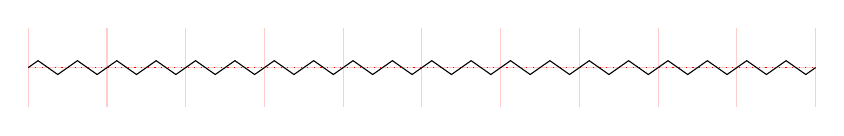
\begin{tikzpicture}[baseline=0pt]
\draw[red!20] (0,-0.5) grid (10,0.5);
\draw[dotted,red] (0,0) -- (10,0);
\draw[decorate,decoration={zigzag,segment length=0.5cm}] (0,0) -- (10,0);
\end{tikzpicture}
& 10pt
\\
\RDD{segment length}=2cm
&  
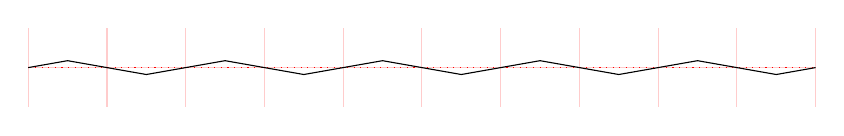
\begin{tikzpicture}[baseline=0pt]
\draw[red!20] (0,-0.5) grid (10,0.5);
\draw[dotted,red] (0,0) -- (10,0); \draw[decorate,decoration={zigzag,segment length=2cm}] (0,0) -- (10,0);
\end{tikzpicture}
& 
\\ \hline  
\RDD{amplitude}=0.5cm
&  
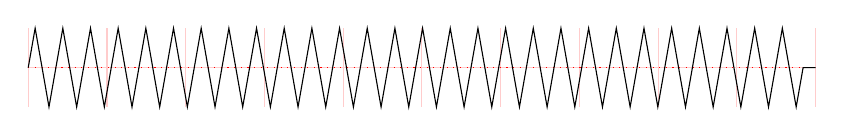
\begin{tikzpicture}[baseline=0pt]
\draw[red!20] (0,-0.5) grid (10,0.5);
\draw[dotted,red] (0,0) -- (10,0); \draw[decorate,decoration={zigzag,amplitude=0.5cm}] (0,0) -- (10,0);
\end{tikzpicture}
& 2.5 pt
\\ \hline 
\end{tabular}

\bigskip

\begin{tabular}{|c|c|c|} \hline 
 \multicolumn{3}{|c|}{ \BSS{draw}[decorate,decoration= 
 \AC{saw,\RDD{segment length}=20pt }] (1,1) circle (1);}
  \\ \hline  
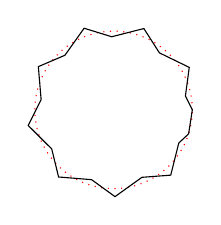
\begin{tikzpicture}
\draw [dotted,red](1,1) circle (1);
\draw [decorate,decoration={zigzag,segment length=20pt}]
(1,1) circle (1); 
\end{tikzpicture}
&  
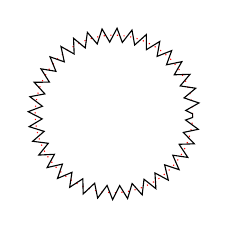
\begin{tikzpicture}
\draw [dotted,red](1,1) circle (1);
\draw [decorate,decoration={zigzag,segment length=5pt}]
(1,1) circle (1); 
\end{tikzpicture}
&  
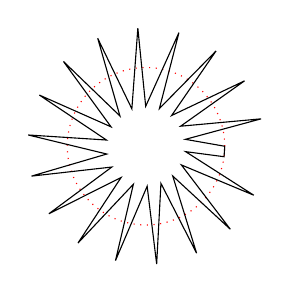
\begin{tikzpicture}
\draw [dotted,red](1,1) circle (1);
\draw [decorate,decoration={zigzag,amplitude=0.5cm}]
(1,1) circle (1); 
\end{tikzpicture}
\\ \hline 
\RDD{segment length}=20pt & \RDD{segment length}=5pt & \RDD{amplitude}=0.5cm 
\\ \hline 
\end{tabular}


\subsubsection{\og bent \fg }

\begin{tabular}{|c|c|c|} \hline  
\begin{tikzpicture}
\draw [dotted,red](0,0) -- (2,2) ;
\draw [decorate,decoration=bent]
(0,0) -- (2,2) ;
\end{tikzpicture}
&  
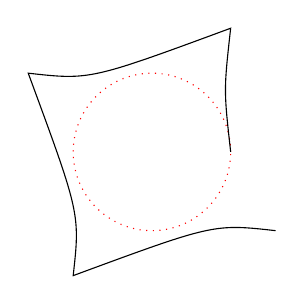
\begin{tikzpicture}
\draw [dotted,red] (1,1) circle (1);
\draw [decorate,decoration=bent]
(1,1) circle (1); 
\end{tikzpicture}
&  
\begin{tikzpicture}
\draw [dotted,red]
(0,0)  arc (0:180:3 and 2);
\draw [decorate,decoration=bent]
(0,0)  arc (0:180:3 and 2);
\end{tikzpicture}
\\ \hline  
(0,0) - - (2,2) & (1,1) circle (1) & (0,0)  arc (0:180:3 and 2); \\ 
\hline 
\end{tabular}

\bigskip

\begin{tabular}{|l|c|c|} \hline 
\multicolumn{2}{|c|}{\BSS{draw}[decorate,decoration=\AC{bent,\RDD{amplitude}=0.5cm}] (0,0) -- (10,0);} & \dft
 \\ \hline 
\RDD{amplitude}=0.5cm
&  
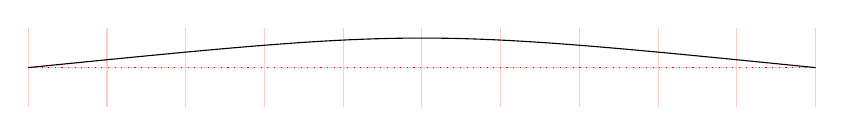
\begin{tikzpicture}[baseline=0pt]
\draw[red!20] (0,-0.5) grid (10,0.5);
\draw[dotted,red] (0,0) -- (10,0); \draw[decorate,decoration={bent,amplitude=0.5cm}] (0,0) -- (10,0);
\end{tikzpicture}
& 2.5 pt
\\ \hline  
\parbox{4cm}{
\RDD{aspect}=0.1 (en bleue)\\
\RDD{aspect}=0.9 (en vert)\\
amplitude=0.5cm\\
}
&  
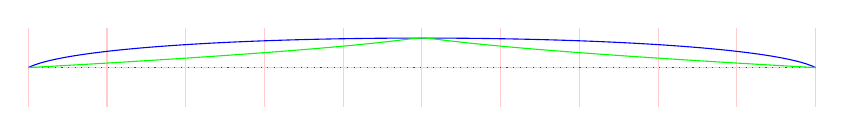
\begin{tikzpicture}[baseline=0pt]
\draw[red!20] (0,-0.5) grid (10,0.5);
\draw[dotted,red] (0,0) -- (10,0); \draw[decorate,blue,decoration={bent,aspect=0.1,amplitude=0.5cm}] (0,0) -- (10,0);
\draw[decorate,green,decoration={bent,aspect=0.9,amplitude=0.5cm}] (0,0) -- (10,0);
\end{tikzpicture}
& 0.5
\\ \hline 
\end{tabular}

\bigskip

\begin{tabular}{|c|c|c|} \hline  
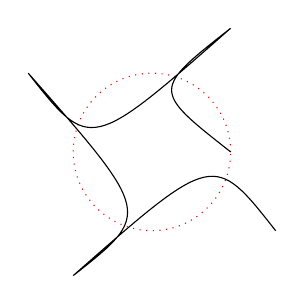
\begin{tikzpicture}
\draw [dotted,red](1,1) circle (1);
\draw [decorate,decoration={bent,amplitude=1cm}]
(1,1) circle (1); 
\end{tikzpicture}
&  
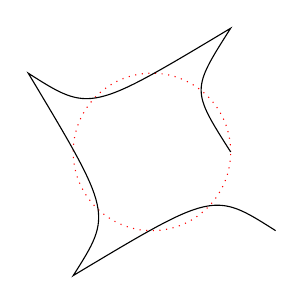
\begin{tikzpicture}
\draw [dotted,red](1,1) circle (1);
\draw [decorate,decoration={bent,amplitude=0.5cm}]
(1,1) circle (1); 
\end{tikzpicture}
&  
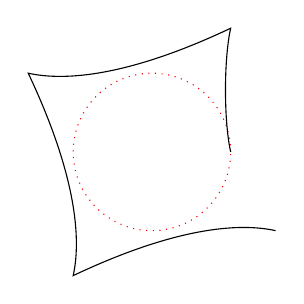
\begin{tikzpicture}
\draw [dotted,red](1,1) circle (1);
\draw [decorate,decoration={bent,aspect=.25}]
(1,1) circle (1); 
\end{tikzpicture}
\\ \hline 
amplitude=1cm & amplitude=0.5cm & aspect=0.25
\\ \hline 
\end{tabular}


\subsubsection{\og bumps \fg  }

\begin{tabular}{|c|c|c|} \hline
\multicolumn{3}{|c|}{\BSS{draw}[decorate,\RDD{decoration}=\RDDX{bumps}{decoration}] (0,0) - - (2,2) ;}
 \\ \hline 
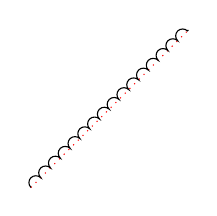
\begin{tikzpicture}
\draw [dotted,red](0,0) -- (2,2) ;
\draw [decorate,decoration=bumps]
(0,0) -- (2,2) ;
\end{tikzpicture}
&  
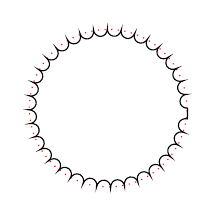
\begin{tikzpicture}
\draw [dotted,red] (1,1) circle (1);
\draw [decorate,decoration=bumps]
(1,1) circle (1); 
\end{tikzpicture}
&  
\begin{tikzpicture}
\draw [dotted,red]
(0,0)  arc (0:180:3 and 2);
\draw [decorate,decoration=bumps]
(0,0)  arc (0:180:3 and 2);
\end{tikzpicture}
\\ \hline  
(0,0) - - (2,2) & (1,1) circle (1) & (0,0)  arc (0:180:3 and 2) \\ 
\hline 
\end{tabular}

\bigskip

\begin{tabular}{|l|c|c|} \hline 
\multicolumn{2}{|c|}{\BSS{draw}[decorate,decoration=\AC{bumps,\RDD{amplitude}=0.5cm}] (0,0) - - (10,0);} & \dft
 \\ \hline 
\RDD{amplitude}=0.5cm
&  
\begin{tikzpicture}[baseline=0pt]
\draw[red!20] (0,-0.5) grid (10,0.5);
\draw[dotted,red] (0,0) -- (10,0); \draw[decorate,decoration={bumps,amplitude=0.5cm}] (0,0) -- (10,0);
\end{tikzpicture}
& 2.5 pt
\\ \hline  
\RDD{segment length}=1cm
&  
\begin{tikzpicture}[baseline=0pt]
\draw[red!20] (0,-0.5) grid (10,0.5);
\draw[dotted,red] (0,0) -- (10,0); \draw[decorate,decoration={bumps,segment length=1cm}] (0,0) -- (10,0);
\end{tikzpicture}
& 10 pt
\\ \hline 
\end{tabular}

\bigskip

\begin{tabular}{|c|c|c|} \hline 
\multicolumn{3}{|c|}{ \BSS{draw}[decorate,decoration= 
\AC{bumps,\RDD{amplitude}=10pt}] (1,1) circle (1);}
 \\ \hline 
\begin{tikzpicture}
\draw [dotted,red](1,1) circle (1);
\draw [decorate,decoration={bumps,amplitude=10pt}]
(1,1) circle (1); 
\end{tikzpicture}
&  
\begin{tikzpicture}
\draw [dotted,red](1,1) circle (1);
\draw [decorate,decoration={bumps,amplitude=0.5cm}]
(1,1) circle (1); 
\end{tikzpicture}
&  
\begin{tikzpicture}
\draw [dotted,red](1,1) circle (1);
\draw [decorate,decoration={bumps,segment length=20pt}] (1,1) circle (1); 
\end{tikzpicture}
\\ \hline 
\RDD{amplitude}=10pt & \RDD{amplitude}=0.5cm & \RDD{segment length}=20pt
\\ \hline 
\end{tabular}


\subsubsection{\og coil \fg }

\begin{tabular}{|c|c|c|} \hline 
\multicolumn{3}{|c|}{\BSS{draw}[decorate,\RDD{decoration}=\RDDX{coil}{decoration}] (0,0) - - (2,2) ;}
 \\ \hline  
\begin{tikzpicture}
\draw [dotted,red](0,0) -- (2,2) ;
\draw [decorate,decoration=coil]
(0,0) -- (2,2) ;
\end{tikzpicture}
&  
\begin{tikzpicture}
\draw [dotted,red] (1,1) circle (1);
\draw [decorate,decoration=coil]
(1,1) circle (1); 
\end{tikzpicture}
&  
\begin{tikzpicture}
\draw [dotted,red]
(0,0)  arc (0:180:3 and 2);
\draw [decorate,decoration=coil]
(0,0)  arc (0:180:3 and 2);
\end{tikzpicture}
\\ \hline  
(0,0) - - (2,2) & (1,1) circle (1) & (0,0)  arc (0:180:3 and 2) \\ 
\hline 
\end{tabular}

\bigskip

\begin{tabular}{|l|c|c|} \hline 
\multicolumn{2}{|c|}{\BSS{draw}[decorate,decoration=\AC{coil,\RDD{amplitude}=0.5cm}] (0,0) - - (10,0);} & \dft
 \\ \hline 
\RDD{amplitude}=0.5cm
&  
\begin{tikzpicture}[baseline=0pt]
\draw[red!20] (0,-0.5) grid (10,0.5);
\draw[dotted,red] (0,0) -- (10,0); \draw[decorate,decoration={coil,amplitude=0.5cm}] (0,0) -- (10,0);
\end{tikzpicture}
& 2.5 pt
\\ \hline  
\RDD{segment length}=1cm
&  
\begin{tikzpicture}[baseline=0pt]
\draw[red!20] (0,-0.5) grid (10,0.5);
\draw[dotted,red] (0,0) -- (10,0);
\draw[decorate,decoration={coil,segment length=1cm}] (0,0) -- (10,0);
\end{tikzpicture}
& 10 pt 
\\ \hline
\parbox{4cm}{

\RDD{aspect}=0.1\\
(amplitude=0.5cm)\\
}
&  
\begin{tikzpicture}[baseline=0pt]
\draw[red!20] (0,-0.5) grid (10,0.5);
\draw[dotted,red] (0,0) -- (10,0);
\draw[decorate,decoration={coil,aspect=0.1,amplitude=0.5cm}] (0,0) -- (10,0);
\end{tikzpicture}
& 
\\
\RDD{aspect}=0.3
&  
\begin{tikzpicture}[baseline=0pt]
\draw[red!20] (0,-0.5) grid (10,0.5);
\draw[dotted,red] (0,0) -- (10,0);
\draw[decorate,decoration={coil,aspect=0.3,amplitude=0.5cm}] (0,0) -- (10,0);
\end{tikzpicture}
&  0.5
\\
\RDD{aspect}=0.9
& 
\begin{tikzpicture}[baseline=0pt]
\draw[red!20] (0,-0.5) grid (10,0.5);
\draw[dotted,red] (0,0) -- (10,0);
\draw[decorate,decoration={coil,aspect=0.9,amplitude=0.5cm}] (0,0) -- (10,0);
\end{tikzpicture}
& 
\\ \hline
\end{tabular}

\bigskip

\begin{tabular}{|c|c|c|} \hline  
\multicolumn{3}{|c|}{ \BSS{draw}[decorate,decoration= \AC{coil,\RDD{amplitude}=0.5cm}] (1,1) circle (1);}
 \\ \hline 
\begin{tikzpicture}
\draw [dotted,red](1,1) circle (1);
\draw [decorate,decoration={coil,amplitude=0.5cm}]
(1,1) circle (1); 
\end{tikzpicture}
&  
\begin{tikzpicture}
\draw [dotted,red](1,1) circle (1);
\draw[decorate,decoration={coil,segment length=1cm,amplitude=0.5cm}]
(1,1) circle (1); 
\end{tikzpicture}
&  
\begin{tikzpicture}
\draw [dotted,red](1,1) circle (1);
\draw [decorate,decoration={coil,aspect=.25,amplitude=0.5cm}]
(1,1) circle (1); 
\end{tikzpicture}
\\ \hline 
\RDD{amplitude}=0.5 cm & \RDD{segment length}=1cm & \RDD{aspect}=0.25 \\
& amplitude=0.5cm & amplitude=0.5cm
\\ \hline 
\end{tabular}

\subsubsection{\og curveto \fg }

\begin{tabular}{|c|c|c|} \hline  
\begin{tikzpicture}
\draw [dotted,red](0,0) -- (2,2) ;
\draw [decorate,decoration=curveto]
(0,0) -- (2,2) ;
\end{tikzpicture}
&  
\begin{tikzpicture}
\draw [dotted,red] (1,1) circle (1);
\draw [decorate,decoration=curveto]
(1,1) circle (1); 
\end{tikzpicture}
&  
\begin{tikzpicture}
\draw [dotted,red];
\draw [decorate,decoration=curveto] (0,0)  arc (0:180:3 and 2);
\end{tikzpicture}
\\ \hline  
(0,0) - - (2,2) & (1,1) circle (1) & (0,0)  arc (0:180:3 and 2) 
\\ \hline 
\end{tabular}


\subsubsection{\og snake \fg }

\begin{tabular}{|c|c|c|} \hline 
\multicolumn{3}{|c|}{\BSS{draw}[decorate,\RDD{decoration}=\RDDX{snake}{decoration}] (0,0) - - (2,2) ;}
 \\ \hline   
\begin{tikzpicture}
\draw [dotted,red](0,0) -- (2,2) ;
\draw [decorate,decoration=snake]
(0,0) -- (2,2) ;
\end{tikzpicture}
&  
\begin{tikzpicture}
\draw [dotted,red] (1,1) circle (1);
\draw [decorate,decoration=snake]
(1,1) circle (1); 
\end{tikzpicture}
&  
\begin{tikzpicture}
\draw [dotted,red]
(0,0)  arc (0:180:3 and 2);
\draw [decorate,decoration=snake]
(0,0)  arc (0:180:3 and 2);
\end{tikzpicture}
\\ \hline  
(0,0) - - (2,2) & (1,1) circle (1) &(0,0)  arc (0:180:3 and 2) \\ 
\hline 
\end{tabular}

\bigskip

\begin{tabular}{|l|c|c|} \hline 
\multicolumn{2}{|c|}{\BSS{draw}[decorate,decoration=\AC{snake,\RDD{segment length}=2cm}] (0,0) - - (10,0);} & \dft
 \\ \hline 
\RDD{amplitude}=0.5cm
&  
\begin{tikzpicture}[baseline=0pt]
\draw[red!20] (0,-0.5) grid (10,0.5);
\draw[dotted,red] (0,0) -- (10,0); \draw[decorate,decoration={snake,amplitude=0.5cm}] (0,0) -- (10,0);
\end{tikzpicture}
& 2.5 pt
\\ \hline  
\RDD{segment length}=1cm
&  
\begin{tikzpicture}[baseline=0pt]
\draw[red!20] (0,-0.5) grid (10,0.5);
\draw[dotted,red] (0,0) -- (10,0);
\draw[decorate,decoration={snake,segment length=1cm}] (0,0) -- (10,0);
\end{tikzpicture}
& 10 pt
\\ \hline  
\end{tabular}

\bigskip

\begin{tabular}{|c|c|c|} \hline  
\multicolumn{3}{|c|}{ \BSS{draw}[decorate,decoration=
snake,
\RDD{amplitude}=5pt] (1,1) circle (1);}
 \\ \hline
\begin{tikzpicture}
\draw [dotted,red](1,1) circle (1);
\draw [decorate,decoration={snake,amplitude=5pt}]
(1,1) circle (1); 
\end{tikzpicture}
&  
\begin{tikzpicture}
\draw [dotted,red](1,1) circle (1);
\draw [decorate,decoration={snake,amplitude=0.5cm}]
(1,1) circle (1); 
\end{tikzpicture}
&  
\begin{tikzpicture}
\draw [dotted,red](1,1) circle (1);
\draw [decorate,decoration={snake,,segment length=1cm}]
(1,1) circle (1); 
\end{tikzpicture}
\\ \hline 
\RDD{amplitude}=5pt & \RDD{amplitude}=0.5cm & \RDD{segment length}=5pt
\\ \hline 
\end{tabular}

\newpage
\subsection{Library \og decorations.pathreplacing \fg}


 \maboite{\BS{usetikzlibrary}\AC{decorations.pathreplacing}}
\label{lib-replac}

\begin{center}
\RRR{48-3}
\end{center}

\subsubsection{\og border \fg }

\begin{tabular}{|c|c|c|} \hline
\multicolumn{3}{|c|}{\BSS{draw}[decorate,\RDD{decoration}=\RDDX{border}{decoration}] (0,0) - - (2,2) ;}
 \\ \hline 
\begin{tikzpicture}
\draw [dotted,red](0,0) -- (2,2) ;
\draw [decorate,decoration=border]
(0,0) -- (2,2) ;
\end{tikzpicture}
&  
\begin{tikzpicture}
\draw [dotted,red] (1,1) circle (1);
\draw [decorate,decoration=border]
(1,1) circle (1); 
\end{tikzpicture}
&  
\begin{tikzpicture}
\draw [dotted,red]
(0,0)  arc (0:180:3 and 2);
\draw [decorate,decoration=border]
(0,0)  arc (0:180:3 and 2);
\end{tikzpicture}
\\ \hline  
(0,0) - - (2,2) & (1,1) circle (1) & (0,0)  arc (0:180:3 and 2) \\ 
\hline 
\end{tabular}

\bigskip

\begin{tabular}{|l|c|c|} \hline 
\multicolumn{2}{|c|}{\BSS{draw}[decorate,decoration=\AC{border,\RDD{amplitude}=0.5cm}] (0,0) - - (10,0);} & \dft
 \\ \hline 
\RDD{amplitude}=0.5cm
&  
\begin{tikzpicture}[baseline=0pt]
\draw[red!20] (0,-0.5) grid (10,0.5);
\draw[dotted,red] (0,0) -- (10,0); \draw[decorate,decoration={border,amplitude=0.5cm}] (0,0) -- (10,0);
\end{tikzpicture}
& 2.5 pt
\\ \hline  
\parbox{4cm}{
\RDD{segment length}=1cm ,\\
amplitude=0.5cm}
&  
\begin{tikzpicture}[baseline=0pt]
\draw[red!20] (0,-0.5) grid (10,0.5);
\draw[dotted,red] (0,0) -- (10,0); \draw[decorate,decoration={border,segment length=1cm,amplitude=0.5cm}] (0,0) -- (10,0);
\end{tikzpicture}
& 10 pt
\\ \hline
\parbox{4cm}{
\RDD{angle}=90 ,\\
amplitude=0.5cm
}
&  
\begin{tikzpicture}[baseline=0pt]
\draw[red!20] (0,-1) grid (10,1);
\draw[dotted,red] (0,0) -- (10,0); \draw[decorate,decoration={border,angle=90,amplitude=0.5cm}] (0,0) -- (10,0);
\end{tikzpicture}
& 45
\\ \hline 
\end{tabular}

\bigskip

\begin{tabular}{|c|c|c|} \hline  
\multicolumn{3}{|c|}{ \BSS{draw}[decorate,decoration=
\AC{border,\RDD{amplitude}=0.5cm}] (1,1) circle (1);}
\\ \hline 
\begin{tikzpicture}
\draw [decorate,decoration={border,amplitude=0.5cm}]
 (1,1) circle (1); 
\end{tikzpicture}
 & 
\begin{tikzpicture}
\draw [dotted,red](1,1) circle (1);
\draw [decorate,decoration={border,segment length=1cm,amplitude=0.5cm}]
(1,1) circle (1); 
\end{tikzpicture}
&  
\begin{tikzpicture}
\draw [dotted,red](1,1) circle (1);
\draw [decorate,decoration={border,angle=90,amplitude=0.5cm}]
(1,1) circle (1); 
\end{tikzpicture}
\\ \hline 
 \RDD{amplitude}=0.5cm & \RDD{segment length}=1cm &\RDD{angle}=90 \\
 & ,amplitude=0.5cm & ,amplitude=0.5cm
\\ \hline 

\end{tabular}

\subsubsection{\og brace \fg }

\begin{tabular}{|c|c|} \hline 
\begin{tikzpicture}[baseline=0pt]
\draw [decorate,decoration=brace] (0,0) -- (3,0);
\end{tikzpicture}
 &  
 \BS{draw} [decorate,\RDD{decoration}=\RDDX{brace}{decoration}] (0,0) - - (3,1);
 \\ \hline 
\end{tabular} 

\bigskip

\begin{tabular}{|c|c|c|c|} \hline 
\multicolumn{3}{|c|}{ \BSS{draw}[decorate,decoration=
\AC{brace,\RDD{amplitude}=0.5cm}] (1,1) circle (1); ;}
\\ \hline 
\begin{tikzpicture}
\draw [dotted,red](0,0) -- (2,2) ;
\draw [decorate,decoration={brace,amplitude=0.5cm}](0,0) -- (2,2) ;
\end{tikzpicture}
&  
\begin{tikzpicture}
\draw [dotted,red](0,0) -- (2,2) ;
\draw [decorate,decoration={brace,aspect=.65,amplitude=0.5cm}]
(0,0) -- (2,2) ; 
\end{tikzpicture}
&  
\begin{tikzpicture}
\draw [dotted,red](0,0) -- (2,2) ;
\draw [decorate,decoration={brace,raise=0.25cm,amplitude=0.5cm}]
(0,0) -- (2,2) ;
\end{tikzpicture}
&
\begin{tikzpicture}
\draw [dotted,red](0,0) -- (2,2) ;
\draw [decorate,decoration={brace,mirror,amplitude=0.5cm}]
(0,0) -- (2,2) ;
\end{tikzpicture}
\\ \hline 
\RDD{amplitude}=0.5cm & \RDD{aspect}=0.65 & \RDD{raise}= 0.25cm & \RDD{mirror}
\\ 
					& ,amplitude = 0.5cm & ,amplitude = 0.5cm& ,amplitude = 0.5cm
\\ \hline  
\dft : 2.5 & \dft : 0.5 &  \dft : 0 & \\ 
\hline 
\end{tabular}

\subsubsection{\fg expanding waves \fg }

\begin{tabular}{|c|c|} \hline  
\begin{tikzpicture}[baseline=0pt]
\draw [dotted,red](0,0) -- (2,0) ;
\draw [dashed,red](0,0) -- (20:2) ;
\draw [dashed,red](0,0) -- (-20:2) ;
\draw [decorate,decoration={expanding waves}](0,0) -- (2,0) ;
\end{tikzpicture}
&  
\parbox{10cm}{
\BS{draw} [dashed,red](0,0) - - (20:2) ;\\
\BS{draw} [dashed,red](0,0) - - (-20:2) ;\\
\BS{draw} [decorate,decoration=\AC{\RDD{expanding waves}}](0,0) - - (2,0) ;
}
\\ \hline 
\end{tabular} 

\bigskip

\begin{tabular}{|c|c|} \hline
\multicolumn{2}{|c|}{ \BSS{draw}[decorate,decoration=
\AC{expanding waves,\RDD{segment length}=0.5cm}] (1,1) circle (1);}
\\ \hline 
\begin{tikzpicture}
\draw [dotted,red](0,0) -- (2,2) ;
\draw [decorate,decoration={expanding waves,segment length=0.5cm}](0,0) -- (2,2) ;
\end{tikzpicture}
&  
\begin{tikzpicture}
\draw [dotted,red](0,0) -- (2,2) ;
\draw [decorate,decoration={expanding waves,angle=45}]
(0,0) -- (2,2) ;
\end{tikzpicture}
\\ \hline 
\RDD{segment length}=0.5cm & \RDD{angle}=45
\\ \hline 
 
\dft : 10pt &  \dft : 20\\ 
\hline 
\end{tabular}

\subsubsection{\og moveto \fg }
 
 \TFRGB{voir}{see} page \pageref{moveto}

\subsubsection{\og  ticks \fg }

\begin{tabular}{|c|c|c|} \hline 
\multicolumn{3}{|c|}{\BSS{draw}[decorate,\RDD{decoration}=\RDDX{ticks}{decoration}] (0,0) - - (2,2) ;}
 \\ \hline  
\begin{tikzpicture}
\draw [dotted,red](0,0) -- (2,2) ;
\draw [decorate,decoration=ticks]
(0,0) -- (2,2) ;
\end{tikzpicture}
&  
\begin{tikzpicture}
\draw [dotted,red] (1,1) circle (1);
\draw [decorate,decoration=ticks]
(1,1) circle (1); 
\end{tikzpicture}
&  
\begin{tikzpicture}
\draw [dotted,red]
(0,0)  arc (0:180:3 and 2);
\draw [decorate,decoration=ticks]
(0,0)  arc (0:180:3 and 2);
\end{tikzpicture}
\\ \hline  
(0,0) - - (2,2) & (1,1) circle (1) & (0,0)  arc (0:180:3 and 2) \\ 
\hline 
\end{tabular}
 \bigskip

\begin{tabular}{|l|c|c|} \hline 
\multicolumn{2}{|c|}{\BSS{draw}[decorate,decoration=\AC{ticks,\RDD{amplitude}=0.5cm}] (0,0) - - (10,0);} & \dft
 \\ \hline 
\RDD{amplitude}=0.5cm
&  
\begin{tikzpicture}[baseline=0pt]
\draw[red!20] (0,-1) grid (10,1);
\draw[dotted,red] (0,0) -- (10,0); \draw[decorate,decoration={ticks,amplitude=0.5cm}] (0,0) -- (10,0);
\end{tikzpicture}
& 2.5 pt
\\ \hline  
\RDD{segment length}=1cm
&  
\begin{tikzpicture}[baseline=0pt]
\draw[red!20] (0,-0.5) grid (10,0.5);
\draw[dotted,red] (0,0) -- (10,0); \draw[decorate,decoration={ticks,segment length=1cm}] (0,0) -- (10,0);
\end{tikzpicture}
& 10 pt
\\ \hline
\end{tabular}

\bigskip

\begin{tabular}{|c|c|c|} \hline 
\multicolumn{3}{|c|}{ \BSS{draw}[decorate,decoration=
\AC{ticks,\RDD{segment length}=1cm}] (1,1) circle (1); }
 \\ \hline  
\begin{tikzpicture}
\draw [dotted,red] (1,1) circle (1); 
\draw [decorate,decoration={ticks,segment length=1cm}](1,1) circle (1); 
\end{tikzpicture}
&  
\begin{tikzpicture}
\draw [dotted,red](1,1) circle (32pt); 
\draw [decorate,decoration={ticks,segment length=pi*8}](1,1) circle (32pt); 
\end{tikzpicture}
&  
\begin{tikzpicture}
\draw [dotted,red](1,1) circle (1); 
\draw [decorate,decoration={ticks,amplitude=0.5cm}]
(1,1) circle (1); 
\end{tikzpicture}
\\ \hline 
\RDD{segment length}=1cm & segment length=\RDD{pi*8} & \RDD{amplitude}=0.5cm \\
(1,1) circle (1) & (1,1) circle (32pt) & (1,1) circle (1)
\\ \hline 
\end{tabular}

\subsubsection{\fg waves \fg }

\begin{tabular}{|c|c|c|} \hline 
\multicolumn{3}{|c|}{\BSS{draw}[decorate,\RDD{decoration}=\RDDX{waves}{decoration}] (0,0) - - (2,2) ;}
 \\ \hline  
\begin{tikzpicture}
\draw [dotted,red](0,0) -- (2,2) ;
\draw [decorate,decoration=waves]
(0,0) -- (2,2) ;
\end{tikzpicture}
&  
\begin{tikzpicture}
\draw [dotted,red] (1,1) circle (1);
\draw [decorate,decoration=waves]
(1,1) circle (1); 
\end{tikzpicture}
&  
\begin{tikzpicture}
\draw [dotted,red]
(0,0)  arc (0:180:3 and 2);
\draw [decorate,decoration=waves]
(0,0)  arc (0:180:3 and 2);
\end{tikzpicture}
\\ \hline  
(0,0) - - (2,2) & (1,1) circle (1) & (0,0)  arc (0:180:3 and 2)\\ 
\hline 
\end{tabular}

\bigskip

\begin{tabular}{|l|c|c|} \hline 
\multicolumn{2}{|c|}{\BSS{draw}[decorate,decoration=\AC{waves,\RDD{angle}=60,radius=1cm}] (0,0) - - (10,0);} & \dft
 \\ \hline 
\RDD{angle}=60
&  
\begin{tikzpicture}[baseline=0pt]
\draw[red!20] (0,-0.5) grid (10,0.5);
\draw[dotted,red] (0,0) -- (10,0); \draw[decorate,decoration={waves,angle=60,radius=1cm}] (0,0) -- (10,0);
\end{tikzpicture}
& 45
\\ \hline  
\RDD{segment length}=1cm
&  
\begin{tikzpicture}[baseline=0pt]
\draw[red!20] (0,-0.5) grid (10,0.5);
\draw[dotted,red] (0,0) -- (10,0); \draw[decorate,decoration={waves,segment length=1cm,radius=1cm}] (0,0) -- (10,0);
\end{tikzpicture}
& 10 pt
\\ \hline
\RDD{radius}=2cm
&  
\begin{tikzpicture}[baseline=0pt]
\draw[red!20] (0,-0.5) grid (10,0.5);
\draw[dotted,red] (0,0) -- (10,0); \draw[decorate,decoration={waves,radius=2cm}] (0,0) -- (10,0);
\end{tikzpicture}
& 10 pt
\\ \hline
\end{tabular}

\bigskip

\begin{tabular}{|c|c|c|} \hline 
\multicolumn{3}{|c|}{ \BSS{draw}[decorate,decoration=
\{waves,\RDD{segment length}=pi*8,} \\
\multicolumn{3}{|c|}{radius=1cm\}] (1,1) circle (32pt); }
 \\ \hline  
\begin{tikzpicture}
\draw [dotted,red](1,1) circle (32pt); 
\draw [decorate,decoration={waves,segment length=pi*8,radius=1cm}]
(1,1) circle (32pt); 
\end{tikzpicture}
&  
\begin{tikzpicture}
\draw [dotted,red](1,1) circle (32pt); 
\draw [decorate,decoration={waves,angle=60,segment length=pi*8,radius=1cm}]
(1,1) circle (32pt); 
\end{tikzpicture}
&  
\begin{tikzpicture}
\draw [dotted,red](1,1) circle (32pt); 
\draw [decorate,decoration={waves,segment length=pi*8,radius=2cm}]
(1,1) circle (32pt); 
\end{tikzpicture}
\\ \hline 
\RDD{segment length} = pi*8 & \RDD{angle}=60 & \RDD{radius}=2cm \\
& , segment length = pi*8 & , segment length = pi*8
\\ \hline 
\end{tabular}

\subsubsection{\og show path construction \fg }


\begin{tabular}{|l|} \hline 
\multicolumn{1}{|c|}{ \emph{\TFRGB{Chemin à décorer}{path to decorate}} }
\\ \hline  
\BS{draw} [blue,dashed] (0,0) - - (2,1)  arc (-20:135:1) - - cycle \\
(3,2)   .. controls (7,0) and (2,0) .. (5,2) - - (6,2) sin (7.57,0)  - - (8,3) ;
\\ \hline 
\begin{tikzpicture}
\draw [blue,dashed] (0,0) -- (2,1)  arc (-20:135:1) -- cycle (3,2)   .. controls (7,0) and (2,0) .. (5,2) -- (6,2) sin (7.57,0)  -- (8,3) ;
\end{tikzpicture} 
\\ \hline 
\end{tabular} 

\bigskip


\begin{tabular}{|l|} \hline 
\multicolumn{1}{|c|}{ \textbf{\TFRGB{composantes linéaires  }{ Linear components} : \og  lineto \fg  }  }
\\ \hline 
 
decoration=\{ \RDD{show path construction},\\
\RDD{lineto code}=\AC{ \BS{draw} [red,ultra thick,->] \\ (\BSS{tikzinputsegmentfirst}) - - (\BSS{tikzinputsegmentlast});
},\}
\\ \hline 
\begin{tikzpicture}
\draw [blue,dashed] (0,0) -- (2,1)  arc (-20:135:1) -- cycle (3,2)   .. controls (7,0) and (2,0) .. (5,2) -- (6,2) sin (7.57,0)  -- (8,3) ;
\path [decorate,decoration={show path construction,lineto code={
\draw [red,ultra thick,->] (\tikzinputsegmentfirst) -- (\tikzinputsegmentlast);
},} ]  (0,0) -- (2,1)  arc (-20:135:1) -- cycle (3,2)   .. controls (7,0) and (2,0) .. (5,2) -- (6,2) sin (7.57,0)  -- (8,3) ;;
\end{tikzpicture} 
\\ \hline 
\end{tabular} 

\bigskip


\begin{tabular}{|l|} \hline 
\multicolumn{1}{|c|}{ \textbf{\TFRGB{Fermetures de chemin }{ Path terminations} : \og  closepath \fg  }  }
\\ \hline  
decoration=\{ \RDD{show path construction},\\
\RDD{closepath code}=\AC{ \BS{draw} [red,ultra thick,->] \\ (\BSS{tikzinputsegmentfirst}) - - (\BSS{tikzinputsegmentlast});
},\}
\\ \hline 
\begin{tikzpicture}
\draw [blue,dashed] (0,0) -- (2,1)  arc (-20:135:1) -- cycle (3,2)   .. controls (7,0) and (2,0) .. (5,2) -- (6,2) sin (7.57,0)  -- (8,3) ;
\path [decorate,decoration={show path construction,closepath code={
\draw [red,ultra thick,->] (\tikzinputsegmentfirst) -- (\tikzinputsegmentlast);
},} ]  (0,0) -- (2,1)  arc (-20:135:1) -- cycle (3,2)   .. controls (7,0) and (2,0) .. (5,2) -- (6,2) sin (7.57,0)  -- (8,3) ;
\end{tikzpicture} 
\\ \hline 
\end{tabular} 

\bigskip


\begin{tabular}{|l|} \hline 
\multicolumn{1}{|c|}{ \textbf{\TFRGB{coupure de chemin }{ Broken paths} : \og  moveto \fg  }  }
\\ \hline  
decoration=\{ \RDD{show path construction},\\
\RDD{moveto code}=\AC{ \BS{draw} [red,ultra thick,->] \\ (\BSS{tikzinputsegmentfirst}) - - (\BSS{tikzinputsegmentlast});
},\}
\\ \hline 
\begin{tikzpicture}
\draw [blue,dashed] (0,0) -- (2,1)  arc (-20:135:1) -- cycle (3,2)   .. controls (7,0) and (2,0) .. (5,2) -- (6,2) sin (7.57,0)  -- (8,3) ;
\path [decorate,decoration={show path construction,moveto code={
\draw [red,ultra thick,->] (\tikzinputsegmentfirst) -- (\tikzinputsegmentlast);
},} ]  (0,0) -- (2,1)  arc (-20:135:1) -- cycle (3,2)   .. controls (7,0) and (2,0) .. (5,2) -- (6,2) sin (7.57,0)  -- (8,3) ;
\end{tikzpicture} 
\\ \hline 
\end{tabular} 

\newpage
 

\begin{tabular}{|l|} \hline 
\multicolumn{1}{|c|}{ \textbf{\TFRGB{composants courbes }{ Curved segments} : \og  curveto \fg  }  }
\\ \hline  
decoration=\{ \RDD{show path construction},\\
\RDD{curveto code}=\AC{ \BS{draw} [red,ultra thick,->] \\ (\BSS{tikzinputsegmentfirst}) - - (\BSS{tikzinputsegmentlast});
},\}
\\ \hline 
\begin{tikzpicture}
\draw [blue,dashed] (0,0) -- (2,1)  arc (-20:135:1) -- cycle (3,2)   .. controls (7,0) and (2,0) .. (5,2) -- (6,2) sin (7.57,0)  -- (8,3) ;
\path [decorate,decoration={show path construction,curveto code={
\draw [red,ultra thick,->] (\tikzinputsegmentfirst) -- (\tikzinputsegmentlast);
},} ]  (0,0) -- (2,1)  arc (-20:135:1) -- cycle (3,2)   .. controls (7,0) and (2,0) .. (5,2) -- (6,2) sin (7.57,0)  -- (8,3) ;
\end{tikzpicture} 
\\ \hline 

\hline  
decoration=\{ \RDD{show path construction},\\
\RDD{curveto code}=\AC{ \BS{draw} [red,ultra thick,->] \\ (\BSS{tikzinputsegmentfirst}) - - (\BSS{tikzinputsegmentsupporta});
},\}
\\ \hline 
\begin{tikzpicture}
\draw [blue,dashed] (0,0) -- (2,1)  arc (-20:135:1) -- cycle (3,2)   .. controls (7,0) and (2,0) .. (5,2) -- (6,2) sin (7.57,0)  -- (8,3) ;
\path [decorate,decoration={show path construction,curveto code={
\draw [red,ultra thick,->] (\tikzinputsegmentfirst) -- (\tikzinputsegmentsupporta);
},} ]  (0,0) -- (2,1)  arc (-20:135:1) -- cycle (3,2)   .. controls (7,0) and (2,0) .. (5,2) -- (6,2) sin (7.57,0)  -- (8,3) ;
\end{tikzpicture} 
\\ \hline 

\hline  
decoration=\{ \RDD{show path construction},\\
\RDD{curveto code}=\AC{ \BS{draw} [red,ultra thick,->] \\ (\BSS{tikzinputsegmentlast}) - - (\BSS{tikzinputsegmentsupportb});
},\}
\\ \hline 
\begin{tikzpicture}
\draw [blue,dashed] (0,0) -- (2,1)  arc (-20:135:1) -- cycle (3,2)   .. controls (7,0) and (2,0) .. (5,2) -- (6,2) sin (7.57,0)  -- (8,3) ;
\path [decorate,decoration={show path construction,curveto code={
\draw [red,ultra thick,->] (\tikzinputsegmentlast) -- (\tikzinputsegmentsupportb);
},} ]  (0,0) -- (2,1)  arc (-20:135:1) -- cycle (3,2)   .. controls (7,0) and (2,0) .. (5,2) -- (6,2) sin (7.57,0)  -- (8,3) ;
\end{tikzpicture} 
\\ \hline 
\hline  
decoration=\{ \RDD{show path construction},\\
\RDD{curveto code}=\AC{ \BS{draw} [red,ultra thick,->] \\ (\BSS{tikzinputsegmentfirst}) .. controls  (\BSS{tikzinputsegmentsupporta}) \\
and (\BSS{tikzinputsegmentsupportb}) .. (\BSS{tikzinputsegmentlast})
;
},\}
\\ \hline 
\begin{tikzpicture}
\draw [blue,dashed] (0,0) -- (2,1)  arc (-20:135:1) -- cycle (3,2)   .. controls (7,0) and (2,0) .. (5,2) -- (6,2) sin (7.57,0)  -- (8,3) ;
\path [decorate,decoration={show path construction,curveto code={
\draw [red,ultra thick,->] (\tikzinputsegmentfirst) .. controls (\tikzinputsegmentsupporta) and (\tikzinputsegmentsupportb) .. (\tikzinputsegmentlast);} } ]  
(0,0) -- (2,1)  arc (-20:135:1) -- cycle (3,2)  -- (6,2) sin (7.57,0)  -- (8,3) ;
\end{tikzpicture} 
\\ \hline 
.. controls (7,0) and (2,0) .. (5,2) \DW{} 
\\ \hline 
\end{tabular}


\newpage


\subsection{Library \og decorations.markings \fg }

 \maboite{\BS{usetikzlibrary}\AC{decorations.markings}}
\label{lib-mark}

\begin{center}
\RRR{48-4}
\end{center}

\SbSbSSCT{Sa marque à une position}{Personal mark at one position}

\begin{tabular}{|c|} \hline  
\BS{draw} [decorate,decoration=\{markings,\RDD{mark}=\RDDX{at position}{mark} 1cm \\ \RDD{ with} \{ 
\textbf{\BS{draw}[red] (-2pt,-2pt) - - (2pt,2pt);} 
\textbf{\BS{draw}[red](2pt,-2pt) - - (-2pt,2pt);}\\
\textbf{\BS{draw}[red] (-2pt,-2pt) rectangle (2pt,2pt); }
\}\}] (1,1) circle (1);
\\ \hline  
\begin{tikzpicture}
\draw[dotted] (1,1) circle (1);
\draw [decorate,decoration={markings,mark=at position 1cm with {
\draw[red] (-2pt,-2pt) -- (2pt,2pt);
\draw[red] (2pt,-2pt) -- (-2pt,2pt);
\draw[red] (-2pt,-2pt) rectangle (2pt,2pt);
}}]
(1,1) circle (1);
\end{tikzpicture}
\\ \hline 
\end{tabular} 

\SbSbSSCT{Ses marques : origine, fin et  pas }{Marks between positions with step size}


\begin{tabular}{|c|c|} \hline 
\multicolumn{2}{|c|}{\BSS{draw}[decorate,\{markings,mark=\RDD{between positions} 0 \RDD{and} 1  \RDD{step} 5mm with ... \}] (1,1) circle (1);;}
\\ \hline   
\begin{tikzpicture}
\draw[dotted] (1,1) circle (1);
\draw [decorate,decoration={markings,mark=between positions 0 and 1 step 5mm with {
\draw[red] (-2pt,-2pt) -- (2pt,2pt);
\draw[red] (2pt,-2pt) -- (-2pt,2pt);
\draw[red] (-2pt,-2pt) rectangle (2pt,2pt);
}}]
(1,1) circle (1);
\end{tikzpicture}
&  
\begin{tikzpicture}
\draw[dotted] (1,1) circle (1);
\draw [decorate,decoration={markings,mark=between positions 0 and 0.5 step 5mm with {
\draw[red] (-2pt,-2pt) -- (2pt,2pt);
\draw[red] (2pt,-2pt) -- (-2pt,2pt);
\draw[red] (-2pt,-2pt) rectangle (2pt,2pt);
}}]
(1,1) circle (1);
\end{tikzpicture}
\\ \hline  
mark=\RDD{between positions} 0 \RDD{and} 1  \RDD{step} 5mm &
  \RDD{between positions} 0 \RDD{and} 0.5  \RDD{step} 5mm
\\ \hline 
\begin{tikzpicture}
\draw[dotted] (1,1) circle (1);
\draw [decorate,decoration={markings,mark=between positions 0 and 1 step 1/10 with {
\draw[red] (-2pt,-2pt) -- (2pt,2pt);
\draw[red] (2pt,-2pt) -- (-2pt,2pt);
\draw[red] (-2pt,-2pt) rectangle (2pt,2pt);
}}]
(1,1) circle (1);
\end{tikzpicture}
&  
\begin{tikzpicture}
\draw[dotted] (1,1) circle (1);
\draw [decorate,decoration={markings,mark=between positions 0 and 1 step .1 with {
\draw[red] (-2pt,-2pt) -- (2pt,2pt);
\draw[red] (2pt,-2pt) -- (-2pt,2pt);
\draw[red] (-2pt,-2pt) rectangle (2pt,2pt);
}}]
(1,1) circle (1);
\end{tikzpicture}
\\ \hline  
mark= \RDD{between positions} 0 \RDD{and} 1 \RDD{step} 1/10 &
	\RDD{between positions} 0 \RDD{and} 1  \RDD{step}0.1
\\ \hline

\end{tabular} 

\bigskip

\SbSbSSCT{Marque avec un n\oe ud contenant du texte}{Marks with a text node}

\begin{tabular}{|c|c|c|} \hline  
\multicolumn{3}{|c|}{
decoration=\AC{markings,mark=at position 1cm with {\color{red}{\BS{node}[red]}\AC{texte}}}}
\\ \hline  
\begin{tikzpicture}
\draw[dotted] (1,1) circle (1);
\draw [decorate,decoration={markings,mark=at position 1cm with \node[red]{texte};
}]
(1,1) circle (1);
\end{tikzpicture}
&  
\begin{tikzpicture}
\draw[dotted] (1,1) circle (1);
\draw [decorate,decoration={markings,mark=at position 0.5 with \node[red]{texte};
}]
(1,1) circle (1);
\end{tikzpicture}
&  
\begin{tikzpicture}
\draw[dotted] (1,1) circle (1);
\draw [decorate,decoration={markings,mark=at position -1cm with \node[red]{texte};
}]
(1,1) circle (1);
\end{tikzpicture}
\\ \hline  
at position 1cm & at position 0.5 & at position -1cm 
\\ \hline 
\begin{tikzpicture}
\draw[dotted] (1,1) circle (1);
\draw [decorate,decoration={markings,mark=at position 1cm/2 with \node[red]{texte};
}]
(1,1) circle (1);
\end{tikzpicture}
&  
\begin{tikzpicture}
\draw[dotted] (1,1) circle (1);
\draw [decorate,decoration={markings,mark=at position 0.5/2 with \node[red]{texte};
}]
(1,1) circle (1);
\end{tikzpicture}
&  
\begin{tikzpicture}
\draw[dotted] (1,1) circle (1);
\draw [decorate,decoration={markings,mark=at position -.3 with \node[red]{texte};
}]
(1,1) circle (1);
\end{tikzpicture}
\\ \hline  
at position 1cm/2 & at position 0.5/2 & at position -0.5/2 
\\ \hline 

\end{tabular} 
 \bigskip

\SbSbSSCT{Marque avec un n\oe ud contenant une image}
{Mark with a picture node}

\begin{tabular}{|c|c|} \hline
\multicolumn{2}{|c|}{
\BS{draw} [decorate,decoration=\AC{markings,mark=at position 1cm with {\color{red}{\BS{node}\AC{\BS{DFR}}}};
}]
(1,1) circle (1);}
\\  \hline
\begin{tikzpicture}
\draw[dotted] (1,1) circle (1);
\draw [decorate,decoration={markings,mark=at position 1cm with \node{\DFR};
}]
(1,1) circle (1);
\end{tikzpicture}
&  
\begin{tikzpicture}
\draw[dotted] (1,1) circle (1);
\draw [decorate,decoration={markings,mark=at position 1cm with \node[transform shape]{\DFR};
}]
(1,1) circle (1);
\end{tikzpicture}

\\ \hline  
\BS{node}\AC{\BS{DFR}} &  \BS{node}[\RDD{transform shape}]\AC{\BS{DFR}}
\\ \hline 
\begin{tikzpicture}
\draw[dotted] (1,1) circle (1);
\draw [decorate,decoration={markings,mark=at position 1cm with \node{\includegraphics[width=0.5cm]{tiger}};
}]
(1,1) circle (1);
\end{tikzpicture}
&  
\begin{tikzpicture}
\draw[dotted] (1,1) circle (1);
\draw [decorate,decoration={markings,mark=at position 1cm with \node[transform shape]{\includegraphics[width=0.5cm]{tiger}};
}]
(1,1) circle (1);
\end{tikzpicture}

\\ \hline  
 \BS{node}\{ 
&  
\BS{node}[transform shape]\{ \\
\BS{includegraphics}[width=0.5cm]\AC{tiger} \} 
& 
\BS{includegraphics}[width=0.5cm]\AC{tiger} \}
\\ \hline 
\end{tabular}

\bigskip

\SbSbSSCT{Numérotation des marques et affectation d'un nom }{ Numbered marks}

\begin{tabular}{|c|c|}\hline  
\begin{tikzpicture}[baseline=0pt,decoration={markings,
mark=between positions 0 and 1 step 0.2 with {
\node [red,draw,circle,fill=white,
name=marque-\pgfkeysvalueof{/pgf/decoration/mark info/sequence number},
transform shape]
{\pgfkeysvalueof{/pgf/decoration/mark info/sequence number}};}}]
\draw [postaction={decorate}] (0,0)  arc (180:0:2 and 1.5);
\end{tikzpicture}
& 
\parbox[c]{11cm}{ 
decoration=\{markings,\\
mark=between positions 0 and 1 step 0.2 \\
with \{ \BS{node} [draw , circle ,fill=white, name= \\
{\color{blue} marque-}\BSS{pgfkeysvalueof}\AC{{\color{red}/pgf/decoration/mark info/sequence number}},\\
transform shape] \\
\AC{\BSS{pgfkeysvalueof}\AC{{\color{red}/pgf/decoration/mark info/sequence number}}};\}\}
}
\\ \hline 
\begin{tikzpicture}[baseline=0pt,decoration={markings,
mark=between positions 0 and 1 step 0.2 with {
\node [draw,circle,fill=white,
name=marque-\pgfkeysvalueof{/pgf/decoration/mark info/sequence number},
transform shape]
{\pgfkeysvalueof{/pgf/decoration/mark info/sequence number}};}}]
\draw [postaction={decorate}] (0,0)  arc (180:0:2 and 1.5);
\draw [red,ultra thick] (marque-3) -- (marque-5);
\end{tikzpicture}
& 
\parbox[c]{11cm}{ 
\BS{draw} [red,ultra thick] ({\color{blue}   marque-3}) - - ({\color{blue} marque-5});
}
\\ \hline 
\end{tabular} 

\SbSbSSCT{Distance des n\oe uds }{Marks info}

\begin{tabular}{|c|} \hline 
\begin{tikzpicture}[baseline=0pt,decoration={markings,
mark=between positions 0 and 1 step 40pt with {
\node [red,draw,ellipse,fill=white,font=\tiny]
{ \pgfkeysvalueof{/pgf/decoration/mark info/distance from start}
\pgfkeysvalueof{/pgf/decoration/mark info/mark info/distance from start}
};}}]
\draw [postaction={decorate}] (0,0)  arc (180:0:3 and 2);
\end{tikzpicture}
\\ \hline  
decoration=\{markings,\\
mark=between positions 0 and 1 step 40pt with \\
\{ \BS{node} [red,draw,ellipse,fill=white,font=\BS{tiny}] \\
\AC{\BSS{pgfkeysvalueof}\AC{{\color{red}/pgf/decoration/mark info/distance from start}}
};\} \}
\\ \hline 
\end{tabular}

\bigskip 

/pgf/decoration/reset marks (no value)

/pgf/decoration/mark connection node=node name (no default, initially empty)

\SbSbSSCT{N\oe ud sur une liaison}{Mark with a connection node}

\begin{tabular}{|c|c|} \hline  
\begin{tikzpicture}[baseline=0pt]

\draw [decorate,decoration={markings,
mark connection node=noeud,
mark=at position 0.4 with
{\node [draw,ellipse,blue,transform shape] (noeud) {texte};}}]  (0,0) -- (3,2) ;
\end{tikzpicture}
&  
\parbox[b]{11cm}{
\BS{draw} [decorate,decoration=\{markings,\\
\RDD{mark connection node}={\color{blue}  mon noeud},mark=at position 0.4 with \\
\AC{\BSS{node} [draw,ellipse,blue,transform shape] ({\color{blue}  mon noeud}) \AC{texte};}\}] \\
 (0,0) -- (3,2) ;}
\\ \hline 
\end{tabular}
 
\subsubsection{Arrow Tip Markings}

\begin{tabular}{|c|c|c|c|} \hline  
\multicolumn{4}{|c|}{ \BS{draw}[decorate,decoration=\{ markings,mark=at position 1cm with } \\
\multicolumn{4}{|c|}{\AC{\BSS{arrow}[blue,line width=2mm]{\color{red}\AC{>}}};\}] (1,1) circle (1); }
\\ \hline
\begin{tikzpicture}
\draw [white] (-0.5,-0.5) rectangle (2.5,2.5);
\draw[dotted] (1,1) circle (1);
\draw [decorate,decoration={markings,mark=at position 1cm with {\arrow[blue,line width=2mm]{>}};}] (1,1) circle (1);
\end{tikzpicture}
&  
\begin{tikzpicture}
\draw [white] (-0.5,-0.5) rectangle (2.5,2.5);
\draw[dotted] (1,1) circle (1);
\draw [decorate,decoration={markings,mark=at position 1cm with {\arrow[blue,line width=2mm]{stealth}};}] (1,1) circle (1); 
\end{tikzpicture}
&  
\begin{tikzpicture}
\draw [white] (-0.5,-0.5) rectangle (2.5,2.5);
\draw[dotted] (1,1) circle (1);
\draw [decorate,decoration={markings,mark=at position 1cm with {\arrow[blue,line width=2mm]{|}};
}] (1,1) circle (1);
\end{tikzpicture}
&  
\begin{tikzpicture}
\draw [white] (-0.5,-0.5) rectangle (2.5,2.5);
\draw[dotted] (1,1) circle (1);
\draw [decorate,decoration={markings,mark=at position 1cm with {\arrow[blue,line width=2mm]{diamond}};
}] (1,1) circle (1);
\end{tikzpicture}
\\ \hline  
{\color{red}\AC{>}} & {\color{red}\AC{stealth }}  &{\color{red}\AC{|}}  &{\color{red}\AC{diamond}} \\ 
\hline 
\multicolumn{4}{|c|}{ \TFRGB{Autres possibilités et paramètres voir page \pageref{fleches} et suivantes}{Other possibilities see page \pageref{fleches} } }
\\ \hline 
\end{tabular}

\bigskip

\begin{tabular}{|c|c|c|c|} \hline 
\multicolumn{4}{|c|}{ \BS{draw}[decorate,decoration=\{markings,mark=at position 1cm with } \\
\multicolumn{4}{|c|}{ \AC{\BSS{arrowreversed}[blue,line width=2mm]{\color{red}\AC{>}}};\}] (1,1) circle (1);}
\\ \hline 
\begin{tikzpicture}
\draw [white] (-.5,-.5) rectangle (2.5,2.5);
\draw[dotted] (1,1) circle (1);
\draw [decorate,decoration={markings,mark=at position 1cm with {\arrowreversed[blue,line width=2mm]{>}}; }] (1,1) circle (1);
\end{tikzpicture}
&  
\begin{tikzpicture}
\draw [white] (-.5,-.5) rectangle (2.5,2.5);
\draw[dotted] (1,1) circle (1);
\draw [decorate,decoration={markings,mark=at position 1cm with {\arrowreversed[blue,line width=2mm]{stealth}}; }] (1,1) circle (1);
\end{tikzpicture}
&  
\begin{tikzpicture}
\draw [white] (-.5,-.5) rectangle (2.5,2.5);
\draw[dotted] (1,1) circle (1);
\draw [decorate,decoration={markings,mark=at position 1cm with {\arrowreversed[blue,line width=2mm]{|}}; }] (1,1) circle (1);
\end{tikzpicture}
&  
\begin{tikzpicture}
\draw [white] (-.5,-.5) rectangle (2.5,2.5);
\draw[dotted] (1,1) circle (1);
\draw [decorate,decoration={markings,mark=at position 1cm with {\arrowreversed[blue,line width=2mm]{diamond}}; }] (1,1) circle (1);
\end{tikzpicture}
\\ \hline  
{\color{red}\AC{>}} & {\color{red}\AC{stealth }}   &{\color{red}\AC{|}}  &{\color{red}\AC{diamond}} 
\\ \hline  
\end{tabular} 



\newpage
\subsection{Library \og decorations.footprints \fg }


 \maboite{\BS{usetikzlibrary}\AC{decorations.footprints}}
\label{lib-footprints}

\begin{center}
\RRR{48-5-2}
\end{center}

 \bigskip
\begin{tabular}{|c|} \hline  
\BS{tikz} \BS{draw}[decorate,\RDD{decoration}=\RDDX{footprints}{decoration}] (0,0) -- (10,0);

\\ \hline  
\tikz \draw[decorate,decoration=footprints] (0,0) -- (10,0);

\\ \hline 
\end{tabular} 

 \bigskip

\begin{tabular}{|c|c|c|c|} \hline  
\multicolumn{4}{|c|}{\BSS{draw}[decorate,decoration=\AC{footprints,\RDD{foot of} = \RDDX{gnome}{foot of}}] (0,2.5) - - (3,2.5);}
 \\ \hline  
\tikz \draw[decorate,decoration={footprints,foot of = gnome}] (0,2.5) -- (3,2.5);
&  
\tikz \draw[decorate,decoration={footprints,foot of = human}](0,2.5) -- (3,2.5);
&  
\tikz \draw[decorate,decoration={footprints,foot of = bird}] (0,2.5) -- (3,2.5);
&  

\tikz \draw[decorate,decoration={footprints,foot of = felis silvestris}]  (0,2.5) -- (3,2.5);
\\ \hline  
foot of = \RDDX{gnome}{foot of} & foot of = \RDDX{human}{foot of} & foot of = \RDDX{bird}{foot of} & foot of = \RDDX{felis silvestris}{foot of} \\ 
 & (\dft) & & \\
\hline 
\end{tabular} 

 \bigskip

\begin{tabular}{|c|c|c|c|} \hline  
\multicolumn{4}{|c|}{\BSS{fill}[decorate,decoration=\AC{footprints,foot of = gnome}] (0,2.5) - - (3,2.5);}
 \\ \hline  
\tikz \fill[decorate,decoration={footprints,foot of = gnome}] (0,2.5) -- (3,2.5);
&  
\tikz \fill[decorate,decoration={footprints,foot of = human}](0,2.5) -- (3,2.5);
&  
\tikz \fill[decorate,decoration={footprints,foot of = bird}] (0,2.5) -- (3,2.5);
&  

\tikz \fill[decorate,decoration={footprints,foot of = felis silvestris}]  (0,2.5) -- (3,2.5);
\\ \hline  
foot of = gnome & foot of = human & foot of = bird & foot of = felis silvestris \\ 
\hline 
\end{tabular} 

 \bigskip
\begin{tabular}{|c|c|}\hline  
\multicolumn{2}{|c|}{\BS{fill}[decorate,decoration=\AC{footprints,\RDD{foot length}=20pt}] (0,2.5) - - (3,2.5);}
 \\ \hline 
\begin{tikzpicture}[baseline=0pt]
\draw[red!20] (0,-1) grid (6,1); 
\draw[decorate,decoration={footprints,foot length=1cm}] (0,0) -- (6,0);
\end{tikzpicture} 
&  
\begin{tikzpicture}[baseline=0pt]
\draw[red!20] (0,-1) grid (6,1); 
\draw[decorate,decoration={footprints,stride length=2cm}] (0,0) -- (6,0);
\end{tikzpicture} 

\\ \hline 
 \RDD{foot length}=1cm  &  \RDD{stride length}=2cm  \\ 
\hline 
\dft{} : 10pt & \dft{} : 30pt
 \\ \hline 
\begin{tikzpicture}[baseline=0pt]
\draw[red!20] (0,-1) grid (6,1);
 \draw[decorate,decoration={footprints,foot sep=1cm}] (0,0) -- (6,0);
 \end{tikzpicture} 
&  
\begin{tikzpicture}[baseline=0pt]
\draw[red!20] (0,-1) grid (6,1);
 \draw[decorate,decoration={footprints,foot angle =45}] (0,0) -- (6,0);
\end{tikzpicture} 
\\ \hline 
\RDD{foot sep}=1cm  &  \RDD{foot angle} = 45  \\ 
\hline 
\dft{} : 4pt & \dft{} : 10
 \\ \hline
\end{tabular} 

 \bigskip


\begin{tabular}{|c|c|c|c|}\hline  
\multicolumn{4}{|c|}{\BS{fill}[decorate,decoration=\AC{footprints,\RDD{foot length}=20pt}] (0,2.5) - - (3,2.5);}
 \\ \hline 
\begin{tikzpicture}[baseline=0pt]
\draw[red!20] (0,-0.5) grid (3,0.5); 
\draw[decorate,decoration={footprints,foot length=20pt}] (0,0) -- (3,0);
\end{tikzpicture}
& 
\begin{tikzpicture}[baseline=0pt]
\draw[red!20] (0,-0.5) grid (3,0.5); 
\draw[decorate,decoration={footprints,foot length=1cm}] (0,0) -- (3,0);
\end{tikzpicture} 
&
\begin{tikzpicture}[baseline=0pt]
\draw[red!20] (0,-0.5) grid (3,0.5); 
\draw[decorate,decoration={footprints,stride length=15pt}] (0,0) -- (3,0);
\end{tikzpicture}
&  
\begin{tikzpicture}[baseline=0pt]
\draw[red!20] (0,-0.5) grid (3,0.5); 
\draw[decorate,decoration={footprints,stride length=2cm}] (0,0) -- (3,0);
\end{tikzpicture} 

\\ \hline 
\RDD{foot length}=20pt & \RDD{foot length}=1cm  & \RDD{stride length}=15pt & \RDD{stride length}=2cm  \\ 
\hline 
\multicolumn{2}{|c|}{\dft{} : foot length=10pt} &
\multicolumn{2}{|c|}{\dft{} : stride length=30pt}
 \\ \hline 
\tikz \draw[decorate,decoration={footprints,foot sep=10pt}] (0,2.5) -- (3,2.5);
&  
\tikz \draw[decorate,decoration={footprints,foot sep=1cm}] (0,2.5) -- (3,2.5);
&
\tikz \draw[decorate,decoration={footprints,foot angle = -45}] (0,2.5) -- (3,2.5);
&  
\tikz \draw[decorate,decoration={footprints,foot angle =45}] (0,2.5) -- (3,2.5);

\\ \hline 
\RDD{foot sep}=10pt & \RDD{foot sep}=1cm  & \RDD{foot angle} = -45 & \RDD{foot angle} = 45  \\ 
\hline 
\multicolumn{2}{|c|}{\dft{} : foot sep=4pt} &
\multicolumn{2}{|c|}{\dft{} : foot angle=10}
 \\ \hline
\end{tabular} 


\newpage
\subsection{Library \og decorations.shapes \fg }
\subsubsection{Introduction}


 \maboite{\BS{usetikzlibrary}\AC{decorations.shapes}}
\label{lib-shapes}

\begin{center}
\RRR{48-5-3}
\end{center}
 \bigskip

\begin{center}
\begin{tabular}{|c|c|c|c|} \hline  
\multicolumn{3}{|c|}{\BSS{draw}[decorate,\RDD{decoration}=\RDDX{crosses}{decoration}] (0,0) - - (3,0);}
 \\ \hline  
\tikz \draw[decorate,decoration=crosses] (0,0) -- (3,0);
&  
\tikz \draw[decorate,decoration=triangles] (0,0) -- (3,0);
&  
\tikz \draw[decorate,decoration=shape backgrounds] (0,0) -- (3,0);
\\ \hline  
\RDD{crosses} & \RDD{triangles} & \RDD{shape backgrounds}  \\ 
\hline 
\end{tabular}
\end{center} 

 \bigskip

\begin{tabular}{|l|c|} \hline 
\multicolumn{2}{|c|}{\BSS{draw}[decorate,decoration=\AC{crosses,\RDD{segment length}=1cm}](0,0) -  - (10,0);} 
\\ \hline 

\RDD{segment length} = 1cm
&  
\tikz \draw[decorate,decoration={crosses,segment length=1cm}] (0,0) -- (10,0);
\\ \hline  
\RDD{shape width} = 1cm
&  
\tikz \draw[decorate,decoration={crosses,shape width=1cm}] (0,0) -- (10,0);
\\ \hline  
\RDD{shape height} = 1cm
&  
\tikz \draw[decorate,decoration={crosses,shape
 height=1cm}] (0,0) -- (10,0);
\\ \hline 
\RDD{shape size} = 1cm
&  
\tikz \draw[decorate,decoration={crosses,shape size=1cm}] (0,0) -- (10,0);
\\ \hline 
\multicolumn{2}{|c|}{\dft :  shape width = shape height =  2.5pt}
 \\ \hline 
\end{tabular} 



\subsubsection{\og shape backgrounds \fg }



\tikzset{paint/.style={ draw=#1!50!black, fill=#1!50 },
decorate with/.style=
{decorate,decoration={shape backgrounds,shape=#1,shape size=2mm}}}

\begin{tabular}{|c|c|c|c|} \hline  
 \multicolumn{4}{|c|}{\BS{draw}[\RDD{decorate with}=dart] (0,2.5) - - (3,2.5); }  
 \\ \hline 
\tikz \draw[decorate with=dart] (0,2.5) -- (3,2.5);
&  
\tikz \draw[decorate with=diamond] (0,2.5) -- (3,2.5);
&  
\tikz \draw[decorate with=rectangle] (0,2.5) -- (3,2.5);
&  
\tikz \draw[decorate with=circle] (0,2.5) -- (3,2.5);
\\ \hline 
dart & diamond & rectangle &  circle\\ 
\hline 
\tikz \draw[decorate with=star] (0,2.5) -- (3,2.5);
&  
\tikz \draw[decorate with=regular polygon] (0,2.5) -- (3,2.5);
&  
\tikz \draw[decorate with=signal] (0,2.5) -- (3,2.5);
&  
\tikz \draw[decorate with=kite] (0,2.5) -- (3,2.5);
\\ \hline 
star & regular polygon & signal & kite 
\\ \hline 
\multicolumn{4}{|c|}{\TFRGB{Autres possibilités et paramètres voir page \pageref{formes} et suivantes}{Other possibilities or parameters see from page \pageref{formes} }}

\\ \hline
\end{tabular} 

\bigskip 

\begin{tabular}{|l|c|}\hline 
\multicolumn{2}{|c|}{  \TFRGB{Formes disponibles}{Shapes available} }
\\ \hline 
\emph{\TFRGB{Syntaxe}{Syntax}} &\BSS{draw}[decorate,decoration=\{ \RDD{shape backgrounds},\RDD{shape}=dart,\\
 & shape size=.5cm,shape sep=1cm\}] (0,0) - - (10,0);
 \\ \hline 
\emph{\TFRGB{Autre syntaxe}{Other syntax}}
 &
\BS{draw}[\RDD{decorate with}=dart,decoration=\AC{shape size=.5cm,shape sep=1cm}] \\
 & (0,0) -- (10,0); 
 
 \\ \hline \hline   
\RDD{dart}
&  
\tikz \draw[decorate,decoration={shape backgrounds, shape=dart,shape size=.5cm,shape sep=1cm}] (0,2.5) -- (10,2.5);
\\ \hline  
\RDD{rectangle}
&  
\tikz \draw[decorate,decoration={shape backgrounds, shape=rectangle,shape size=.5cm,shape sep=1cm}] (0,2.5) -- (10,2.5);
\\ \hline 
\RDD{cloud}
&  
\tikz \draw[decorate,decoration={shape backgrounds, shape=cloud,shape size=.5cm,shape sep={1cm}}] (0,2.5) -- (10,2.5);
\\ \hline
\RDD{star}
&  
\tikz \draw[decorate,decoration={shape backgrounds, shape=star,shape size=.5cm,shape sep={1cm}}] (0,2.5) -- (10,2.5);
\\ \hline   
\RDD{starburst}
&  
\tikz \draw[decorate,decoration={shape backgrounds, shape=starburst,shape size=.5cm,shape sep={1cm}}] (0,2.5) -- (10,2.5);
\\ \hline  
\RDD{tape}
&  
\tikz \draw[decorate,decoration={shape backgrounds, shape=tape,shape size=.5cm,shape sep={1cm}}] (0,2.5) -- (10,2.5);
\\ \hline  
\RDD{kite}
&   
\tikz \draw[decorate,decoration={shape backgrounds, shape=kite,shape size=.5cm,shape sep={1cm}}] (0,2.5) -- (10,2.5);
\\ \hline 
\RDD{signal}
&   
\tikz \draw[decorate,decoration={shape backgrounds, shape=signal,shape size=.5cm,shape sep={1cm}}] (0,2.5) -- (10,2.5);
\\ \hline 
\multicolumn{2}{|c|}{\dft :   shape= circle }
 \\ \hline
 \multicolumn{2}{|c|}{ \TFRGB{Autres possibilités  voir page \pageref{formes} et suivantes} {Other possibilities see page  \pageref{formes} }}
  \\ \hline 
\end{tabular} 

\bigskip

\begin{tabular}{|c|c|c|c|} \hline
\multicolumn{2}{|c|}{  \TFRGB{Paramètres}{Parameters} }
\\ \hline  
 \multicolumn{4}{|l|}{\BS{draw}[decorate with=star,\RDD{star points}=3,decoration=\AC{shape size=.5cm,shape sep=1cm}]  }\\
 \multicolumn{4}{|l|}{ (0,2.5) - - (3,2.5); } 
 \\ \hline
\tikz \draw[decorate with=star,star points=3,decoration={shape size=.5cm,shape sep=1cm}] (0,2.5) -- (3,2.5);
& 
\tikz \draw[decorate with=star,star points=4,decoration={shape size=.5cm,shape sep=1cm}] (0,2.5) -- (3,2.5);
& 
\tikz \draw[decorate with=star,star points=5,,decoration={shape size=.5cm,shape sep=1cm}] (0,2.5) -- (3,2.5);
&  
\tikz \draw[decorate with=star,star points=8,decoration={shape size=.5cm,shape sep=1cm}] (0,2.5) -- (3,2.5);
\\ \hline  
star points=3 & star points=4 & star points=5 & star points=8\\ \hline 

 \hline 
 \multicolumn{4}{|c|}{\BS{draw}[decorate with=star,\RDD{paint}=green,decoration=\AC{shape size=.5cm,shape sep=1cm}] } \\
\\
 \multicolumn{4}{|l|}{ (0,2.5) - - (3,2.5); }  
 \\ \hline 
\tikz \draw[decorate with=star,paint=green,decoration={shape size=.5cm,shape sep=1cm}] (0,2.5) -- (3,2.5);
&  
\tikz \draw[decorate with=star,double,decoration={shape size=.5cm,shape sep=1cm}] (0,2.5) -- (3,2.5);
&  
\tikz \draw[decorate with=star,star points=8,ultra thick,decoration={shape size=.5cm,shape sep=1cm}] (0,2.5) -- (3,2.5);
&  
\tikz \draw[decorate with=star,star point ratio = 3,decoration={shape size=.5cm,shape sep=1cm}] (0,2.5) -- (3,2.5);
\\ \hline  
\RDD{paint}=green
&  
\RDD{double}
&  
\RDD{ultra thick}
&  
\RDD{star point ratio} = 3
\\ \hline 
\end{tabular} 

\bigskip


\begin{tabular}{|c|c|} \hline
\multicolumn{2}{|c|}{  \TFRGB{Espacement}{Spacing} }
\\ \hline  
 
\multicolumn{2}{|c|}{\BSS{draw}[decorate with=dart,decoration=\{shape size=.5cm,}\\
\multicolumn{2}{|c|}{\RDD{shape sep}=1cm\}] (0,2.5) -  - (10,2.5);}
 \\ \hline 
 
shape sep=\AC{1cm}
&  
\tikz \draw[decorate with=dart,decoration={shape size=.5cm,shape sep=1cm}] (0,2.5) -- (10,2.5);
\\ \hline  
shape sep=\AC{2cm}
&  
\tikz \draw[decorate with=dart,decoration={shape size=.5cm ,shape sep=2cm}] (0,2.5) -- (10,2.5);
\\ \hline 
\multicolumn{2}{|c|}{\dft :  shape sep=                     0.25cm}
 \\ \hline 
\end{tabular} 

\bigskip


\begin{tabular}{|l|c|} \hline 
\multicolumn{2}{|c|}{  \TFRGB{Type d'espacement}{Type of spacing} }
\\ \hline  

\multicolumn{2}{|c|}{\BSS{draw}[decorate with=dart,decoration=\{shape size=.5cm,}\\
\multicolumn{2}{|c|}{
shape sep=\AC{1cm,\RDD{between centers}}\}] (0,2.5) - - (10,2.5);}
 \\ \hline 
\RDD{between centers}
&  
\begin{tikzpicture}
\draw[dotted,red] (0,2.5) -- (10,2.5) ;
\draw[decorate with=dart,decoration={shape size=.5cm,shape sep={1cm,between centers}}] (0,2.5) -- (10,2.5);
\end{tikzpicture}
\\ \hline  
\RDD{between borders}
&  
\begin{tikzpicture}
\draw[dotted,red] (0,2.5) -- (10,2.5) ;
\draw[decorate with=dart,decoration={shape size=.5cm ,shape sep={1cm,between borders}}] (0,2.5) -- (10,2.5);
\end{tikzpicture}
\\ \hline 
\multicolumn{2}{|c|}{\dft :  between centers }
 \\ \hline 
\end{tabular}

\bigskip


\begin{tabular}{|l|c|} \hline
\multicolumn{2}{|c|}{  \TFRGB{Espacement automatique}{Automatic spacing } }
\\ \hline 
 
\multicolumn{2}{|c|}{\BSS{draw}[decorate with=dart,decoration=\{shape size=.5cm,}\\
\multicolumn{2}{|c|}{\RDD{shape evenly spread}=5\}] (0,0) -  - (10,0);}
 \\ \hline 
shape evenly spread=5
&  
\begin{tikzpicture}
\draw[dotted,red] (0,0) -- (10,0) ; \draw[decorate with=dart,decoration={shape size=.5cm,shape evenly spread=5}] (0,0) -- (10,0);
\end{tikzpicture}
\\ \hline  
shape evenly spread=10
&  
\begin{tikzpicture}
\draw[dotted,red] (0,2.5) -- (10,2.5) ;
\draw[decorate with=dart,decoration={shape size=.5cm,shape evenly spread=10}] (0,2.5) -- (10,2.5); 
\end{tikzpicture}

\\ \hline 
\end{tabular} 


\paragraph{Orientation}:


\begin{tabular}{|c|c|} \hline 
\multicolumn{2}{|c|}{ '' shape border rotate `` }
\\ \hline
shape border rotate=90 
& 
\tikz \draw[decorate with=dart,shape border rotate=90,decoration={shape sep=1cm,shape width=.5cm}] (0,0) -- (10,0); 
\\ \hline  
shape border rotate=45
& 
\tikz \draw[decorate with=dart,shape border rotate=45,decoration={shape sep=1cm,shape width=.5cm}] (0,0) -- (10,0); 
\\ \hline  
shape border rotate=180
& 
\tikz \draw[decorate with=dart,shape border rotate=180,decoration={shape sep=1cm,shape width=.5cm}] (0,0) -- (10,0); 
\\ \hline 
\end{tabular} 

 \bigskip


\begin{tabular}{|c|c|} \hline 
\multicolumn{2}{|c|}{ \og shape sloped \fg }
\\ \hline
 \multicolumn{2}{|c|}{\BSS{draw}[decorate with=dart,decoration=\{shape width=.5cm,shape sep=1cm, }\\
 \multicolumn{2}{|c|}{  \RDD{shape sloped}=true \}] (0,0) - - (3,3);}
  \\ \hline
\begin{tikzpicture}
\draw[dotted,red] (0,0) -- (3,3);
\draw[decorate with=dart,decoration={shape width=.5cm ,shape sep=1cm,shape sloped=true}] (0,0) -- (3,3);
\end{tikzpicture}
&  
\begin{tikzpicture}
\draw[dotted,red] (0,0) -- (3,3);
 \draw[decorate with=dart,decoration={shape width=.5cm ,shape sep=1cm,shape sloped=false}] (0,0) -- (3,3);
\end{tikzpicture}
\\ \hline  
shape sloped=true
&  
shape sloped=false
\\ \hline
\multicolumn{2}{|c|}{\dft :  shape sloped=true }
 \\ \hline  
\end{tabular} 
 \bigskip

\begin{tabular}{|c|c|} \hline 
 \multicolumn{2}{|c|}{\BSS{draw}[decorate with=dart,decoration=\{shape width=.5cm,shape sep=1cm, }\\
 \multicolumn{2}{|c|}{  \RDD{shape sloped}=true\}] (0,0)  arc (0:180:3 and 2);}
  \\ \hline
\begin{tikzpicture}
\draw[dotted,red]  (0,0)  arc (0:180:3 and 2);
\draw[decorate with=dart,decoration={shape width=.5cm ,shape sep=1cm,shape sloped=true}] (0,0)  arc (0:180:3 and 2);
\end{tikzpicture}
&  
\begin{tikzpicture}
\draw[dotted,red] (0,0)  arc (0:180:3 and 2);
 \draw[decorate with=dart,decoration={shape width=.5cm ,shape sep=1cm,shape sloped=false}] (0,0)  arc (0:180:3 and 2);
\end{tikzpicture}
\\ \hline  
shape sloped=true
&  
shape sloped=false
\\ \hline
\multicolumn{2}{|c|}{\dft :  shape sloped=true }
 \\ \hline  
\end{tabular} 

 \bigskip

\begin{tabular}{|c|c|} \hline  
 \multicolumn{2}{|c|}{\BSS{draw}[decorate with=dart,decoration=\{shape width=.5cm,shape sep=1cm, }\\
 \multicolumn{2}{|c|}{  \RDD{shape border rotate}=90,shape sloped=true \}] (0,0) - - (3,3);}
  \\ \hline

\begin{tikzpicture}
\draw[dotted,red] (0,0) -- (3,3);
\tikz \draw[decorate with=dart,shape border rotate=90,decoration={shape sep=1cm,shape sloped=true,shape width=.5cm}] (0,0) -- (3,3);
\end{tikzpicture}
&  
\begin{tikzpicture}
\draw[dotted,red] (0,0) -- (3,3);
\draw[decorate with=dart,shape border rotate=90,decoration={shape sep=1cm,shape sloped=false,shape width=.5cm}] (0,0) -- (3,3);
\end{tikzpicture}
\\ \hline  
shape sloped=true
&  
shape sloped=false
\\ \hline
\end{tabular} 

 \bigskip



\begin{tabular}{|c|c|}\hline
\multicolumn{2}{|c|}{ \og shift only \fg }
\\ \hline
 \multicolumn{2}{|c|}{  decoration={
 {\color{red}transform=\AC{shift only}},shape width=5mm,segment length=.5cm,shape sep=1cm}}
  \\ \hline
\begin{tikzpicture}
\draw (0,0)  arc (0:180:3 and 2);
\draw[decorate with=dart,decoration={
transform={shift only},shape width=5mm,segment length=.5cm,shape sep=1cm}]
(0,0)  arc (0:180:3 and 2);
\end{tikzpicture}
& 
\begin{tikzpicture} 
\draw (0,0)  arc (0:180:3 and 2); 
\draw[decorate with=dart,decoration={
shape width=5mm,segment length=.5cm,shape sep=1cm}]
(0,0)  arc (0:180:3 and 2);
\end{tikzpicture}
\\ \hline  
avec &  sans\\ 
\hline 
\end{tabular}


\bigskip

\begin{tabular}{|c|c|} \hline 
\multicolumn{2}{|c|}{ Dimensions }
\\ \hline 
\multicolumn{2}{|c|}{\BSS{draw}[decorate with=dart,decoration=\{shape size=.5cm,}\\
\multicolumn{2}{|c|}{\RDD{shape height}= 1cm \}] (0,0) -  - (10,0);}
\\ \hline 
\RDD{shape height}=1cm
&
\begin{tikzpicture} [baseline=0pt] 
\draw[decorate with=dart,decoration={shape sep=1cm,shape height=1cm}] (0,0) -- (10,0);
\end{tikzpicture}
\\ \hline
\RDD{shape width}=1cm
&
\begin{tikzpicture} [baseline=0pt] 
\draw[decorate with=dart,decoration={shape sep=1cm,shape width=1cm,shape scaled}] (0,0) -- (10,0);
\end{tikzpicture}
\\ \hline 
\RDD{shape size}=1cm
&
\begin{tikzpicture} [baseline=0pt] 
\draw[decorate with=dart,decoration={shape sep=1cm,shape size=1cm,shape scaled}] (0,0) -- (10,0);
\end{tikzpicture}
\\ \hline 
\end{tabular} 


 \bigskip


\begin{tabular}{|l|c|} \hline 
\multicolumn{2}{|c|}{\BSS{draw}[decorate with=dart,decoration=\{shape size=.5cm,}\\
\multicolumn{2}{|c|}{\RDD{shape start size}=1cm,\RDD{shape scaled} \}] (0,2.5) -  - (10,2.5);}
 \\ \hline 
 
\RDD{shape start size}=1cm
&  
\tikz \draw[decorate with=dart,decoration={shape sep=1cm,shape start size=1cm,shape scaled}] (0,0) -- (10,0);
\\ \hline  
\RDD{shape start height}=1cm
&  
\tikz \draw[decorate with=dart,decoration={shape sep=1cm,shape start height=1cm,shape scaled}] (0,0) -- (10,0);

\\ \hline  
\RDD{shape start width}=1cm
&  
\tikz \draw[decorate with=dart,decoration={shape sep=1cm,shape start width=1cm,shape scaled}] (0,0) -- (10,0);
\\ \hline  
\RDD{shape end size}=1cm
&  
\tikz \draw[decorate with=dart,decoration={shape sep=1cm,shape end size=1cm,shape scaled}] (0,0) -- (10,0);

\\ \hline  
\RDD{shape end height}=1cm
&  
\tikz \draw[decorate with=dart,decoration={shape sep=1cm,shape end height=1cm,shape scaled}] (0,0) -- (10,0);
\\ \hline  
\RDD{shape end width}=1cm
&  
\tikz \draw[decorate with=dart,decoration={shape sep=1cm,shape end width=1cm,shape scaled}] (0,0) -- (10,0);
\\ \hline 
\end{tabular} 


\newpage
\subsection{Library \og decorations.text \fg }


 \maboite{\BS{usetikzlibrary}\AC{decorations.text}}
\label{lib-text}

\begin{center}
\RRR{48-6}
\end{center}


\begin{tabular}{|c|} \hline  
 \BS{draw}[decorate,decoration=\AC{{\color{red}text along path,text=\AC{texte}}}] (1,1) circle (1); 
\\ \hline  
\begin{tikzpicture}
\draw[dotted] (1,1) circle (1);
\draw[decorate,decoration={text along path,text={texte}}] (1,1) circle (1); 
\end{tikzpicture}
\\ \hline 
\end{tabular} 


\begin{tabular}{|c|} \hline 
\multicolumn{1}{|c|}{ \TFRGB{Texte trop long}{Text too long} }
\\ \hline 
 
 \BS{draw}[decorate,decoration=\AC{text along path,\\ 
 text=\AC{Un Deux Trois Quatre Cinq Six sept Huit Neuf Dix}}] (1,1) circle (1);
\\ \hline  
\begin{tikzpicture}
\draw[dotted] (1,1) circle (1);
 \draw[decorate,decoration={text along path,text={Un Deux Trois Quatre Cinq Six sept Huit Neuf Dix}}] (1,1) circle (1); 
\end{tikzpicture}
\\ \hline 
\end{tabular} 


\begin{tabular}{|c|c|c|} \hline
\multicolumn{3}{|c|}{ \TFRGB{Format du texte}{Text format}} 
\\ \hline
\multicolumn{3}{|c|}{\BS{draw} [decorate,decoration=\AC{text along path,
text={avant {\color{red}|\BS{red} | texte | |} après }}]}  
\\ \hline
\begin{tikzpicture}
\draw[dotted] (1,1) circle (1);
\draw [decorate,decoration={text along path,
text={avant |\color{red} |texte|| après }}]
(1,1) circle (1);
\end{tikzpicture}
&  
\begin{tikzpicture}
\draw[dotted] (1,1) circle (1);
\draw [decorate,decoration={text along path,
text={|\color{red} |texte||  }}]
(1,1) circle (1);
\end{tikzpicture}
&  
\begin{tikzpicture}
\draw[dotted] (1,1) circle (1);
\draw [decorate,decoration={text along path,
text={|\color{red} |texte|| {} }}]
(1,1) circle (1);
\end{tikzpicture}
\\ \hline  
text=\AC{avant |\BS{red}|texte|| après }  
&  
text=\AC{ |\BS{red}|texte|| } 
&  
text=\AC{ |\BS{red}|texte|| \AC{} } 
\\ \hline 
\end{tabular} 

\bigskip
\begin{tabular}{|c|c|c|} \hline

\begin{tikzpicture}
\draw[dotted] (1,1) circle (1);
\draw [decorate,decoration={text along path,
text={ avant |\color{red}  | texte || après }}]
(1,1) circle (1);
\end{tikzpicture}
&  
\begin{tikzpicture}
\draw[dotted] (1,1) circle (1);
\draw [decorate,decoration={text along path,
text={ avant |\it| texte || après }}]
(1,1) circle (1);
\end{tikzpicture}
&  
\begin{tikzpicture}
\draw[dotted] (1,1) circle (1);
\draw [decorate,decoration={text along path,
text={ avant |\Huge| texte || après }}]
(1,1) circle (1);
\end{tikzpicture}
\\ \hline 
avant | {\color{red} \BS{red}}| texte || après  
& avant | {\color{red}\BS{it}}| texte || après 
& avant | {\color{red}\BS{Huge}}| texte || après  \\ 
\hline 
\end{tabular} 

\bigskip


\begin{tabular}{|c|} \hline  
\BS{draw} [decorate,decoration=\AC{text along path,\\
text=\AC{avant |{\color{red}\BS{Large}}|Visual |{\color{red}+\BS{bf}\BS{color}}\AC{red}|Tikz|| après  }}]
(1,1) circle (1);
\\ \hline  
\begin{tikzpicture}
\draw[dotted] (1,1) circle (1);
\draw [decorate,decoration={text along path,
text={avant |\Large|Visual |+\bf\color{red}|Tikz|| après  }}]
(1,1) circle (1);
\end{tikzpicture}
\\ \hline 
\end{tabular} 


\bigskip

\begin{tabular}{|c|} \hline  
\BS{draw} [decorate,decoration=\AC{text along path,{\color{red}text format delimiters=\AC{[}\AC{]}},\\
text=\AC{ {\color{red} [} \BS{red} {\color{red}  ]} texte {\color{red} [ ]}  }}]
(1,1) circle (1);
\\ \hline  
\begin{tikzpicture}
\draw[dotted] (1,1) circle (1);
\draw [decorate,decoration={text along path,text format delimiters={[}{]},
text={  [ \color{red}  ] texte []  }}]
(1,1) circle (1);
\end{tikzpicture}
\\ \hline 
\end{tabular} 

\bigskip

\begin{tabular}{|c|} \hline
\multicolumn{1}{|c|}{ \TFRGB{Sens du texte}{Text orientation} }
\\ \hline 
\BS{draw}[decorate,decoration=\AC{text along path,text=\AC{texte},\\
text color=blue, \RDD{reverse path} }] (1,1) circle (1);
\\ \hline  
\begin{tikzpicture}
\draw[dotted] (1,1) circle (1);
\draw[decorate,decoration={text along path,text={texte},text color=red}] (1,1) circle (1);
\draw[decorate,decoration={text along path,text={texte},text color=blue, reverse path}] (1,1) circle (1); 
\end{tikzpicture}
\\ \hline 
\end{tabular} 

\bigskip

\begin{tabular}{|c|c|c|} \hline 
\multicolumn{3}{|c|}{ \TFRGB{Position du texte}{Text position} }
\\ \hline  
\multicolumn{3}{|c|}{  \BS{draw}[decorate,decoration=\{ text along path,text=\AC{texte},}\\
\multicolumn{3}{|c|}{  {\color{red}text align=\AC{align=left}}\}] (1,1) circle (1);}  
\\ \hline 
\begin{tikzpicture}
\draw[dotted] (1,1) circle (1);
 \draw[decorate,decoration={text along path,text={texte},text align={align=left}}] (1,1) circle (1); 
\end{tikzpicture}
&  
\begin{tikzpicture}
\draw[dotted] (1,1) circle (1);
 \draw[decorate,decoration={text along path,text={texte},text align={align=center}}] (1,1) circle (1); 
\end{tikzpicture}
&  
\begin{tikzpicture}
\draw[dotted] (1,1) circle (1);
\draw[decorate,decoration={text along path,text={texte},text align={align=right}}] (1,1) circle (1); 
\end{tikzpicture}
\\ \hline  

align=\AC{\RDD{align}=\RDDX{left}{align}} & align=\AC{\RDD{align}=\RDDX{center}{align}} & align=\AC{\RDD{align}=\RDDX{right}{align}} \\ 
\hline 
\end{tabular} 

\bigskip

\begin{tabular}{|c|c|} \hline 
 \multicolumn{2}{|c|}{  \BS{draw}[ decorate,decoration=\{text along path,text=\AC{texte},} \\
 \multicolumn{2}{|c|}{  text align=\AC{align=left,\RDD{left indent}=1cm} \} ] (1,1) circle (1);}  
 \\ \hline 
\begin{tikzpicture}
\draw[dotted] (1,1) circle (1);
\tikz \draw[decorate,decoration={text along path,text={texte},text align={align=left,left indent=1cm}}] (1,1) circle (1); 
\end{tikzpicture}
&  
\begin{tikzpicture}
\draw[dotted] (1,1) circle (1);
\tikz \draw[decorate,decoration={text along path,text={texte},text align={align=right,right indent=1cm}}] (1,1) circle (1); 
\end{tikzpicture}
\\  \hline
 align=\AC{align=left,\RDD{left indent}=1cm}
&  
align=\AC{align=right,\RDD{right indent}=1cm}
 \\ \hline 
\end{tabular} 


\begin{tabular}{|c|} \hline 
\multicolumn{1}{|c|}{ \TFRGB{Justification du texte}{Fit to path} }
\\ \hline 
 
\BS{draw} [decoration=\AC{text along path, text=\AC{Un deux trois quatre },\\
text align=\AC{\RDD{fit to path}}}, decorate]
(1,1) circle (1);
\\ \hline  
\begin{tikzpicture}
\draw[dotted] (1,1) circle (1);
\draw [decoration={text along path, text={Un deux trois quatre },text align={fit to path}}, decorate]
(1,1) circle (1);
\end{tikzpicture}
\\ \hline 
\end{tabular} 



\begin{tabular}{|c|} \hline
\multicolumn{1}{|c|}{ \TFRGB{Justification des espaces}{Fit to path stretching spaces} }
\\ \hline  
\BS{draw} [decoration=\AC{text along path, text=\AC{Un deux trois quatre },\\
text align=\AC{\RDD{fit to path stretching spaces}}}, decorate]
(1,1) circle (1);
 \\ \hline  
\begin{tikzpicture}
\draw[dotted] (1,1) circle (1);
\draw [decoration={text along path, text={Un deux trois quatre },text align={fit to path stretching spaces}}, decorate]
(1,1) circle (1);
\end{tikzpicture}
 \\ \hline 
\end{tabular} 

\newpage

\subsection{Library \og decorations.fractals \fg }


 \maboite{\BS{usetikzlibrary}\AC{decorations.fractals}}
\label{lib-fractals}

\begin{center}
\RRR{48-7}
\end{center}
 \bigskip

\begin{tabular}{|c|c|c|c|} \hline 
\multicolumn{4}{|c|}{\BSS{draw}[decorate,decoration=\RDD{Koch curve type 1}] (0,0) - - (3,0);}
 \\ \hline 
\tikz \draw[decorate,decoration=Koch curve type 1] (0,0) -- (3,0);
 &  
\tikz \draw[decorate,decoration=Koch curve type 2] (0,0) -- (3,0);
 &  
\tikz \draw[decorate,decoration=Koch snowflake] (0,0) -- (3,0);
 &
\tikz \draw[decorate,decoration=Cantor set] (0,0) -- (3,0); 
 \\ \hline  
 
\RDD{Koch curve type 1}  & \RDD{Koch curve type 2}  & \RDD{Koch snowflake} & \RDD{Cantor set} \\ 
\hline 
\end{tabular} 

 \bigskip


\begin{tabular}{|c|c|c|c|} \hline 
\multicolumn{4}{|c|}{\BS{begin}\AC{tikzpicture}[decoration=Koch curve type 1] }
 \\ 
\multicolumn{4}{|c|}{\BS{draw} \color{green}  decorate \AC{ \color{red}  decorate \AC{ \color{black}  (0,0) -- (3,0) \color{red}  }\color{green} };}
 \\ 
\multicolumn{4}{|c|}{\BS{end}\AC{tikzpicture}}  \\  \hline 
\begin{tikzpicture}[decoration=Koch curve type 1]
\draw decorate{ decorate{ (0,0) -- (3,0) }};
\end{tikzpicture}
&  
\begin{tikzpicture}[decoration=Koch curve type 2]
\draw decorate{ decorate{ (0,0) -- (3,0) }};
\end{tikzpicture}
&  
\begin{tikzpicture}[decoration=Koch snowflake]
\draw decorate{ decorate{ ((0,0) -- (3,0) }};
\end{tikzpicture}
&  
\begin{tikzpicture}[decoration=Cantor set]
\draw decorate{ decorate{ (0,0) -- (3,0)}};
\end{tikzpicture}
\\ \hline  &  &  &  \\ 
\hline 
Koch curve type 1  & Koch curve type 2  & Koch snowflake & Cantor set \\ 
\hline 
\end{tabular} 

 \bigskip



\begin{tabular}{|c|c|c|c|} \hline  
\multicolumn{4}{|c|}{\BSS{draw} \color{green} decorate \AC{ \color{red}  decorate \AC{ \color{blue} decorate \AC{ \color{black} (0,0) - - (3,0) \color{blue} } \color{red}  } \color{green}};}
 \\  \hline 
 
\begin{tikzpicture}[decoration=Koch curve type 1]
\draw decorate{ decorate{ decorate{ (0,0) -- (3,0) }}};
\end{tikzpicture}
&  
\begin{tikzpicture}[decoration=Koch curve type 2]
\draw decorate{ decorate{ decorate{ (0,0) -- (3,0) }}};
\end{tikzpicture}
&  
\begin{tikzpicture}[decoration=Koch snowflake ]
\draw decorate{ decorate{ decorate{ (0,0) -- (3,0) }}};
\end{tikzpicture}
&  
\begin{tikzpicture}[decoration=Cantor set]
\draw decorate{ decorate{ decorate{ (0,0) -- (3,0) }}};
\end{tikzpicture}
\\ \hline 
Koch curve type 1  & Koch curve type 2  & Koch snowflake & Cantor set \\ 
\hline 
\end{tabular} 

 \bigskip

\begin{tabular}{|c|c|c|c|} \hline 
\begin{tikzpicture}[decoration=Koch snowflake,draw=blue,fill=blue!20,thick]
\filldraw  (0,0) -- ++(60:3) -- ++(-60:3) -- cycle ;
\end{tikzpicture}
& 
 
\begin{tikzpicture}[decoration=Koch snowflake,draw=blue,fill=blue!20,thick]
\filldraw decorate{ (0,0) -- ++(60:3) -- ++(-60:3) -- cycle };

\end{tikzpicture}
&  
\begin{tikzpicture}[decoration=Koch snowflake,draw=blue,fill=blue!20,thick]
\filldraw decorate{ decorate{ (0,0) -- ++(60:3) -- ++(-60:3) -- cycle }};
\end{tikzpicture}
&  
\begin{tikzpicture}[decoration=Koch snowflake,draw=blue,fill=blue!20,thick]
\filldraw decorate{ decorate{ decorate{ (0,0) -- ++(60:3) -- ++(-60:3) -- cycle }}};
\end{tikzpicture}
\\ \hline  
sans & 1 decorate
&  2 decorate &  3 decorate \\ \hline
\end{tabular}

\newpage


\subsection{Applications}


\SbSbSSCT{Décoration d'un n\oe ud}{Node decoration}

\begin{tabular}{|c|c|} \hline 
 \multicolumn{2}{|c|}{ \BS{node} [draw,decorate,decoration=\{bumps,
  minimum height=2cm, minimum width=3cm\}]
 \AC{texte}; }
  \\  \hline 
\begin{tikzpicture}
\node [fill=green,draw,decorate,decoration={bumps},
 minimum height=2cm, minimum width=3cm,]
{texte};
\end{tikzpicture}
&  
\begin{tikzpicture}
\node [fill=green,draw,decorate,decoration=footprints,
 minimum height=2cm, minimum width=3cm]
{texte};
\end{tikzpicture}
\\ \hline  
decoration=\RDD{bumps}&  decoration=\RDD{footprints} \\ \hline 

\begin{tikzpicture}
\node [fill=green,draw,thick, minimum height=2cm, minimum width=3cm,decorate, decoration={random steps, amplitude=1pt}] {texte};
\end{tikzpicture}
&
\begin{tikzpicture}[decoration={random steps,segment length=3pt , amplitude=2pt}]
\node at (0,0) [fill=green,decorate,starburst,
 minimum height=2cm, minimum width=3cm] {Texte};
\end{tikzpicture}
\\ \hline
 decoration=\{random steps , amplitude = 1pt \} 
 &
  starburst,decoration=\{random steps, \\
  &
 segment length=3pt , amplitude=2pt\} 
\\ \hline 
\begin{tikzpicture}
\node at (0,0) [fill=green,decorate,ellipse,decoration=zigzag,
 minimum height=2cm, minimum width=3cm] {Texte};
\end{tikzpicture}
&  
\begin{tikzpicture}
\node at (0,0) [inner sep=6mm,fill=green,decorate,ellipse,decoration=
{text along path,text={Un Deux Trois Quatre Cinq Six Sept Huit Neuf}}] {texte};
\end{tikzpicture}
\\ \hline  
 ellipse,decoration=zigzag &  decoration= \{text along path,text= \\

 & \AC{Un Deux Trois Quatre Cinq Six Sept Huit Neuf} \}
\\ \hline 
\end{tabular} 

\SbSbSSCT{Décoration de liaisons de noeuds}{Node link decoration}

\begin{tabular}{|c|c|c|} \hline 
\multicolumn{3}{|c|}{\BS{draw} [decorate,decoration=snake](A) -- (B);}
 \\  \hline 
\begin{tikzpicture}[blue]
\node[draw] (A) at (0,0) {A};
\node[draw] (B) at (2,2) {B};
\draw [decorate,decoration=snake](A) -- (B);
\end{tikzpicture}
&  
\begin{tikzpicture}[blue]
\node[draw] (A) at (0,0) {A};
\node[draw] (B) at (2,2) {B};
\draw [decorate,decoration=coil](A) |- (B);
\end{tikzpicture}
&  
\begin{tikzpicture}[blue]
\node[draw] (A) at (0,0) {A};
\node[draw] (B) at (2,2) {B};
\draw [decorate,decoration=footprints](A) -| (B);
\end{tikzpicture}
\\ \hline 
decoration=snake & decoration=coil & decoration=footprints \\
(A){\color{red} - -} (B) & (A) {\color{red}|-} (B) &  (A) {\color{red}-|} (B)
\\ \hline 
\begin{tikzpicture}[blue]
\node[draw] (A) at (0,0) {A};
\node[draw] (B) at (2,2) {B};
\draw [decorate,decoration=coil] (A) to [bend right] (B);
\end{tikzpicture}
&  
\begin{tikzpicture}[blue]
\node[draw] (A) at (0,0) {A};
\node[draw] (B) at (2,2) {B};
\draw[decorate,decoration=zigzag] (A) to[bend left=120]  (B);
\end{tikzpicture} 
&  
\begin{tikzpicture}[blue]
\node[draw] (A) at (0,0) {A};
\node[draw] (B) at (2,2) {B};
\draw [decorate,decoration=ticks](A) to[out=30] (B);
\end{tikzpicture} 
\\ \hline  
decoration=coil & decoration=zigzag & decoration=ticks \\
(A) to [bend right] (B) & (A) to[bend left=120]  (B) & (A) to[out=30] (B)
\\ \hline 

\end{tabular} 

 \bigskip 


\SbSbSSCT{Décoration d'un graphe}{Graph decoration}

\begin{tabular}{|c|c|}\hline 
\multicolumn{2}{|c|}{\BSS{draw}[
\RDD{decorate},decoration=footprints] plot coordinates {(0,0) (2,1) (4,-2)  (6,1) };}
 \\ \hline  
\begin{tikzpicture}[baseline=0pt]
\draw[->,blue] (-.1,0) -- (6,0);
\draw[->,blue] (0,-2.5) -- (0,2.5);
 \draw[red,dashed] plot coordinates {(0,0) (2,1) (4,-2)  (6,1) };
 \draw[decorate,decoration=footprints] plot coordinates {(0,0) (2,1) (4,-2)  (6,1) };
\end{tikzpicture}
&  
\begin{tikzpicture}[domain=0:6.28,x=0.7cm,baseline=0pt]
\draw[->,blue] (-.1,0) -- (7,0);
\draw[->,blue] (0,-2.5) -- (0,2.5);
\draw[red,dashed] plot  (\x,{sin(\x r)});
\draw[decorate,decoration=footprints] plot  (\x,{sin(\x r)});
\end{tikzpicture}
\\ \hline  
plot coordinates {(0,0) (2,1) (4,-2)  (6,1) } 
&
 plot  (\BS{x},\AC{sin(\BS{x} r)})
\\ \hline 
\end{tabular} 


\SbSbSSCT{Décorations variables}{Various decoration}

\begin{tabular}{|c|} \hline 
\BS{draw} [decorate, 
decoration=\AC{zigzag,\RDD{pre}=footprints,\RDD{pre length}=5cm}](0,0) -- (10,0);
\\ \hline  
\begin{tikzpicture}[baseline=0pt]
\draw[red!20] (0,-0.5) grid (10,0.5);
\draw[dotted,red] (0,0) -- (10,0);
\draw [decorate,decoration={zigzag,pre=footprints,pre length=5cm}] (0,0) -- (10,0);
\end{tikzpicture}
\\ \hline  
decoration=\AC{zigzag,\RDD{pre}=footprints,\RDD{pre length}=5cm}
\\ \hline  
\begin{tikzpicture}[baseline=0pt]
\draw[red!20] (0,-0.5) grid (10,0.5);
\draw[dotted,red] (0,0) -- (10,0);
\draw [decorate,decoration={zigzag,post=footprints,post length=5cm}] (0,0) -- (10,0);
\end{tikzpicture}
\\ \hline  
decoration=\AC{zigzag,\RDD{post}=footprints,\RDD{post length}=5cm}
\\ \hline  
\begin{tikzpicture}[baseline=0pt]
\draw[red!20] (0,-0.5) grid (10,0.5);
\draw[dotted,red] (0,0) -- (10,0);
\draw [decorate,decoration={zigzag,pre=footprints,pre length=3cm,post=expanding waves,post length=3cm}] (0,0) -- (10,0);
\end{tikzpicture}
\\ \hline  
decoration=\AC{zigzag,\RDD{pre}=footprints,\RDD{pre length}=3cm,
,\RDD{post}=expanding waves,\RDD{post length}=3cm}
\\ \hline 
\end{tabular} 


\SbSbSSCT{Décoration partielle}{Partial decoration}

\begin{tabular}{|c|l|} \hline  
\begin{tikzpicture}[baseline=0pt]
\draw [decorate,decoration={zigzag}]
 (0,0) -- (2,0) -- (2,1) -- (0,1)-- cycle;
 \end{tikzpicture}
&
\BS{draw} [decorate,decoration=zigzag]
 (0,0) -- (2,0) -- (2,1) -- (0,1)-- cycle;
\\ 
\hline 
  
\begin{tikzpicture}[baseline=0pt]
 \draw  [decoration=zigzag]
 (0,0) -- (2,0) decorate{ -- (2,1)} -- (0,1)-- cycle;
  \end{tikzpicture}
&
\BS{draw} [decoration=zigzag]
 (0,0) -- (2,0) \RDD{decorate}\AC{-- (2,1)} -- (0,1)-- cycle;
\\ 
\hline 
\begin{tikzpicture}[baseline=0pt]
 \draw  [decoration={zigzag}]
 (0,0) -- (2,0)  -- (2,1) decorate{-- (0,1)}-- cycle;
  \end{tikzpicture}
&
\BS{draw} [decorate,decoration=zigzag]
 (0,0) -- (2,0) -- (2,1) -- \RDD{decorate}\AC{(0,1)}-- cycle;
\\ \hline 
\begin{tikzpicture}[baseline=0pt]
 \draw  [decoration={zigzag}]
 (0,0) decorate{-- (2,0)}  -- (2,1) decorate{-- (0,1)}-- cycle;
  \end{tikzpicture}
&
\BS{draw} [decorate,decoration=zigzag]
 (0,0) \RDD{decorate}\AC{-- (2,0)} -- (2,1) -- \RDD{decorate}\AC{(0,1)}-- cycle;
\\ \hline 
 
\end{tabular}

 \newpage



\begin{tabular}{|c|} \hline 
\og lineto \fg
\textbf{}
\BS{draw} [decorate, 
decoration=\AC{zigzag,lineto,\RDD{pre length}=5cm}](0,0) -- (10,0);
\\ \hline  
\begin{tikzpicture}[baseline=0pt]
\draw[red!20] (0,-0.5) grid (10,0.5);
\draw[dotted,red] (0,0) -- (10,0);]
\draw [decorate,decoration={zigzag,pre=lineto,pre length}=5cm] (0,0) -- (10,0);
\end{tikzpicture}
\\ \hline  
decoration=\AC{ zigzag,\RDD{pre}=lineto,\RDD{pre length}=5cm }
\\ \hline  
\begin{tikzpicture}[baseline=0pt]
\draw[red!20] (0,-0.5) grid (10,0.5);
\draw[dotted,red] (0,0) -- (10,0);
\draw [decorate,decoration={zigzag,post=lineto,post length=5cm}] (0,0) -- (10,0);
\end{tikzpicture}
\\ \hline  
decoration=\AC{zigzag,\RDD{post}=lineto,\RDD{post length}=5cm}
\\ \hline  
\begin{tikzpicture}[baseline=0pt]
\draw[red!20] (0,-0.5) grid (10,0.5);
\draw[dotted,red] (0,0) -- (10,0);
\draw [decorate,decoration={zigzag,pre=lineto,pre length=3cm,post=lineto,post length=3cm}] (0,0) -- (10,0);
\end{tikzpicture}
\\ \hline  
decoration=\AC{zigzag,\RDD{pre}=lineto,\RDD{pre length}=3cm,
,\RDD{post}=curveto,\RDD{post length}=3cm}
\\ \hline 
\end{tabular} 


 \bigskip



\begin{tabular}{|c|} \hline 
\og curveto \fg
\\ \hline 
\BS{draw} [decorate, 
decoration=\AC{zigzag,\RDD{pre}=curveto,\RDD{pre length}=5cm}](0,0) -- (10,0);
\\ \hline  
\begin{tikzpicture}[baseline=0pt]
\draw[red!20] (0,-0.5) grid (10,0.5);
\draw[dotted,red] (0,0) -- (10,0);]
\draw [decorate,decoration={zigzag,pre=curveto,pre length=5cm}] (0,0) -- (10,0);
\end{tikzpicture}
\\ \hline  
decoration=\AC{zigzag,\RDD{pre}=curveto,\RDD{pre length}=5cm}
\\ \hline  
\begin{tikzpicture}[baseline=0pt]
\draw[red!20] (0,-0.5) grid (10,0.5);
\draw[dotted,red] (0,0) -- (10,0);
\draw [decorate,decoration={zigzag,post=curveto,post length=5cm}] (0,0) -- (10,0);
\end{tikzpicture}
\\ \hline  
decoration=\AC{zigzag,\RDD{post}=curveto,\RDD{post length}=5cm}
\\ \hline  
\begin{tikzpicture}[baseline=0pt]
\draw[red!20] (0,-0.5) grid (10,0.5);
\draw[dotted,red] (0,0) -- (10,0);
\draw [decorate,decoration={zigzag,pre=curveto,pre length=3cm,post=curveto,post length=3cm}] (0,0) -- (10,0);
\end{tikzpicture}
\\ \hline  
decoration=\AC{zigzag,\RDD{pre}=curveto,\RDD{pre length}=3cm,
,\RDD{post}=curveto,\RDD{post length}=3cm}
\\ \hline 
\end{tabular}

 \bigskip



\label{moveto}
\begin{tabular}{|c|} \hline
\og  moveto \fg 
\\ \hline 
\BS{draw} [decorate, 
decoration=\AC{zigzag,\RDD{pre}=moveto,\RDD{pre length}=5cm}](0,0) -- (10,0);
\\ \hline  
\begin{tikzpicture}[baseline=0pt]
\draw[red!20] (0,-0.5) grid (10,0.5);
\draw[dotted,red] (0,0) -- (10,0);]
\draw [decorate,decoration={zigzag,pre=moveto,pre length=5cm}] (0,0) -- (10,0);
\end{tikzpicture}
\\ \hline  
decoration=\AC{zigzag,\RDD{pre}=moveto,\RDD{pre length}=5cm}
\\ \hline  
\begin{tikzpicture}[baseline=0pt]
\draw[red!20] (0,-0.5) grid (10,0.5);
\draw[dotted,red] (0,0) -- (10,0);
\draw [decorate,decoration={zigzag,post=moveto,post length=5cm}] (0,0) -- (10,0);
\end{tikzpicture}
\\ \hline  
decoration=\AC{zigzag,\RDD{post}=moveto,\RDD{post length}=5cm}
\\ \hline  
\begin{tikzpicture}[baseline=0pt]
\draw[red!20] (0,-0.5) grid (10,0.5);
\draw[dotted,red] (0,0) -- (10,0);
\draw [decorate,decoration={zigzag,pre=moveto,pre length=3cm,post=moveto,post length=3cm}] (0,0) -- (10,0);
\end{tikzpicture}
\\ \hline  
decoration=\AC{zigzag,\RDD{pre}=moveto,\RDD{pre length}=3cm,
,\RDD{post}=moveto,\RDD{post length}=3cm}
\\ \hline 
\end{tabular}

\SbSbSSCT{Paramètres globaux ou particuliers}{Global and  partial parameters }

\begin{tabular}{|l|} \hline  
\begin{tikzpicture}[baseline=0pt,ultra thick,decoration={straight zigzag,amplitude=0.5cm,segment length=1cm}]
\draw[red!20,ultra thin] (0,-2) grid (10,3);
\draw[magenta] (0,2) --  (10,2);
\draw[blue,decorate] (0,1) -- (10,1);
\draw[red,decorate,decoration=saw] (0,0) -- (10,0);
\draw[cyan,decorate,decoration={meta-segment length=2cm}] (0,-1) -- (10,-1);
\end{tikzpicture}

\\ \hline 
\BS{begin}\AC{tikzpicture}[baseline=0pt,ultra thick,\\
{\color{red}decoration=\AC{straight zigzag,amplitude=0.5cm,segment length=1cm}}] \\
\BS{draw}[red!20,ultra thin] (0,-2) grid (10,3); \\
\BS{draw}[magenta] (0,2) --  (10,2); \\
\BS{draw}[blue,\RDD{decorate}] (0,1) -- (10,1); \\
\BS{draw}[red,\AC{\color{red}decorate,decoration=saw}] (0,0) -- (10,0); \\
\BS{draw}[cyan,{\color{red}decorate,decoration={meta-segment length=2cm}}] (0,-1) -- (10,-1); \\
\BS{end}\AC{tikzpicture}

 \\ \hline 
\end{tabular} 


\SbSbSSCT{Tracer le chemin et sa décoration avec  \og  Postaction \fg }{Path and its decoration \og  Postaction \fg }

\begin{tabular}{|c|c|}\hline  
\begin{tikzpicture}[baseline=0pt]
\draw [postaction={decorate,blue,draw,ultra thick,decoration={straight zigzag,amplitude=0.5cm}}][red,line width=10pt] (0,0)  arc (0:180:3 and 2);
\end{tikzpicture}
&  
\parbox[b]{8cm}{
\BS{draw} [\RDD{postaction}=\{decorate,blue,draw,ultra thick, \\
decoration=\AC{straight zigzag,amplitude=0.5cm}\}] \\
 
$[$red,line width = 10pt $]$ (0,0)  arc (0:180:3 and 2);
 
  }
\\ \hline 
\end{tabular} 



\newpage